\documentclass[utf8, russian, hpadding=5mm, vpadding=15mm, floatsection, columnxxvi, columnxxxi, columnxxxii, equationsection, pointsection, footnoteasterisk]{eskdtext}

%доп. пакеты
\usepackage{amsfonts, amsmath, amssymb}	%Для математических штуковин
\usepackage{wallpaper}					%Для вставки сторонних страниц
\usepackage{array}                       %Доп. возможности у таблиц

%доп. настройки
\bibliographystyle{ugost2008}					%Стиль списка литературы
\graphicspath{{./images/}{./extra_pdf_pages/}}	%Папки с картинками

%на случай, если команда не определена
\newcommand{\No}{\textnumero}

%определения своих команд
\DeclareMathOperator{\atan2}{atan2}
\newcommand{\msf}[1]{\mathsf{#1}}    %определение короткого обозначения для спец. начертания в формулах
\newcommand{\nv}{\mathbf0}           %нулевой вектор

%для определения форматирования нумерации элементов списка литературы
\makeatletter
\renewcommand{\@biblabel}[1]{#1}
\makeatother

%для штампа
\ESKDtitle{\normalsize Разработка системы управления для манипулятора Kuka Youbot\\[\smallskipamount]\small Пояснительная записка}
\ESKDsignature{КСУИ.101.4135.001 ПЗ}
\ESKDgroup{\footnotesize Университет ИТМО\\Кафедра СУиИ\\гр.~P4135}
\ESKDauthor{\resizebox{2.22cm}{\height}{Антонов, Артемов}}
\ESKDchecker{\resizebox{2.22cm}{\height}{Котельников Ю.П.}}
\ESKDnormContr{}
\ESKDapprovedBy{}

%оступы от заголовков разделов и подразделов
\ESKDsectSkip{section}{7mm}{7mm}
\ESKDsectSkip{subsection}{5mm}{5mm}
\ESKDsectSkip{subsubsection}{3mm}{3mm}


%тело документа
\begin{document}
%\addtocounter{page}{1} %если в документ будут вставлены иные страницы (ТЗ и проч.)
\ESKDthisStyle{empty}
\mbox{}
\ThisLRCornerWallPaper{1}{title_page_1.pdf}
\newpage
%\ESKDthisStyle{empty}
%\mbox{}
%\ThisLRCornerWallPaper{1}{title_page2.pdf}
%\newpage

\ESKDthisStyle{formII}
\tableofcontents
\newpage
\topmargin = 0 mm
\section*{Обозначения и сокращения}
\addcontentsline{toc}{section}{Обозначения и сокращения}
Используемые далее по тексту общие обозначения:
\newcommand*{\ditem}[1]{\item[#1~---]}
\begin{itemize}
\ditem{СК} система координат;
\ditem{КП} кинематическая пара;
\ditem{ДХ} Денавита-Хартенберга (Denavit–Hartenberg), например, соглашение;
\ditem{ИСО} инерциальная система отсчета;
\ditem{ПЗК} прямая задача кинематики;
\ditem{ОЗК} обратная задача кинематики;
\ditem{$n$} количество звеньев робота, $n = 5$;
\ditem{$q_i$} $i$-ая ($i=\overline{1,n}$) обобщенная координата манипулятора (угол, регистрируемый энкодером робота в $i$-ом сочленении);
\ditem{$q$} вектор-столбец обобщенных координат робота, $q = \left[ q_1 \; q_2 \; q_3 \; q_4 \; q_5 \right]^T$;
\ditem{${}^iR_j$} матрица поворота, характеризующая поворот СК $Ox_{j}y_{j}z_{j}$ относительно СК $Ox_{i}y_{i}z_{i}$;
\ditem{${}^iA_j$} матрица однородного преобразования, описывающая смещение и поворот СК $Ox_{j}y_{j}z_{j}$ относительно СК $Ox_{i}y_{i}z_{i}$\footnote{За пояснениями обратитесь к Приложению~\ref{app_ht_matrices}};
\ditem{$r^i_{j,\,k}$} вектор из начала $Ox_{j}y_{j}z_{j}$ в начало $Ox_{k}y_{k}z_{k}$, выраженный относительно $Ox_{i}y_{i}z_{i}$\footnote{За пояснениями к применяемой здесь и далее терминологии, касающейся относительных измерений, обратитесь к Приложению~\ref{app_relative_relativity}.};
\ditem{$g_i$} ускорение свободного падения, выраженное относительно $Ox_{i}y_{i}z_{i}$;
\ditem{$v^i_j$} линейная скорость начала $Ox_{j}y_{j}z_{j}$ относительно используемой в решении ИСО\lefteqn,\footnote{В~качестве ИСО в документе используется $Ox_0y_0z_0$.} выраженная относительно $Ox_{i}y_{i}z_{i}$;
\ditem{$a^i_j$} линейное ускорение начала $Ox_{j}y_{j}z_{j}$ относительно ИСО, выраженное относительно $Ox_{i}y_{i}z_{i}$;
\ditem{$\omega^i_j$} угловая скорость вращения $Ox_{j}y_{j}z_{j}$ относительно ИСО, выраженная относительно $Ox_{i}y_{i}z_{i}$;
\ditem{$\omega^i_{j,\,k}$} угловая скорость вращения $Ox_{k}y_{k}z_{k}$ относительно $Ox_{j}y_{j}z_{j}$, выраженная относительно $Ox_{i}y_{i}z_{i}$;
\ditem{$\dot\omega^i_j$} угловое ускорение $Ox_{j}y_{j}z_{j}$ относительно ИСО, выраженное относительно $Ox_{i}y_{i}z_{i}$;
\ditem{$z^i_j$} орт $[0\;0\;1]^T$ системы координат $Ox_{j}y_{j}z_{j}$, выраженный относительно $Ox_{i}y_{i}z_{i}$;
\ditem{$f^i_j$} сила, действующая на $j$-ое звено (тело) механизма со стороны $(j-1)$-го звена (тела), выраженная относительно $Ox_{i}y_{i}z_{i}$;
\ditem{$\tau^i_j$} момент силы, действующий на $j$-ое звено (тело) механизма со стороны ${(j-1)}$-го звена (тела), выраженный относительно $Ox_{i}y_{i}z_{i}$;
\ditem{$\tau_i$} обобщенный момент, ответственный за изменение обобщенной координаты $q_i$;
\ditem{$m_i$} масса $i$-го звена;
\ditem{$\mathcal{I}^i_j$} тензор инерции $j$-го звена относительно $Ox_{i}y_{i}z_{i}$;
\ditem{$a_i, d_i$} обозначения для длин, входящих в число параметров Де\-на\-ви\-та-Хар\-тен\-бер\-га, $i=\overline{1,n}$;
\ditem{$\alpha_i, \theta_i$} обозначения для углов, входящих в число параметров Де\-на\-ви\-та-Хар\-тен\-бер\-га, $i=\overline{1,n}$;
\ditem{$s_\gamma, c_\gamma$} синус и косинус угла $\gamma$ соответственно;
\ditem{$s_i, c_i$} синус и косинус угла $\theta_i$ соответственно.
\end{itemize}
\newpage

\section*{Введение}
\addcontentsline{toc}{section}{Введение}
В~данном документе будет рассказано о процессе разработки системы управления для манипулятора робота Kuka Youbot~\cite{technomatix_kuka_youbot}, дающей ему возможность для совершения двух действий: занятия позиции, при которой его схват будет принимать заданные положение и ориентацию, а также перемещения схвата по заданной траектории\footnote{Здесь и далее, когда речь будет идти о траектории движении схвата, под последней будет подразумеваться не просто кривая, описываемая при этом схватом в пространстве, но таковая, явно параметризованная временем.}.
В~целом содержание пояснительной записки можно описать примерно так:
\begin{itemize}
\item в~разделе~\ref{part_description_of_robot} будут приведены технические сведения о роботе, необходимые для решения поставленных задач;
\item раздел~\ref{part_math_model_of_robot} расскажет о процессе составления математической модели манипулятора, а именно о решении применительно к нему прямой и обратной задач кинематики и о составлении дифференциальных уравнений, описывающих протекающие в роботе электрические и механические процессы;
\item в~разделе~\ref{part_control_systems} речь пойдет о синтезе соответствующих систем управления, о проверке их работоспособности с помощью моделирования, о результатах аппробации на реальном роботе и проч.
\end{itemize}
\newpage

\section{Описание манипулятора}\label{part_description_of_robot}
Рассматриваемый в данной работе манипулятор робота Kuka Youbot представляет собой пятизвенный манипулятор, снабженный двухпальцевым схватом.
Описание его массогабаритных параметров дается таблицей~\ref{table_gen_info_of_manipulator} и рисунком~\ref{img:sizes_of_robot}.
Неуказанные там параметры робота, требуемые для дальнейших расчетов, неизвестны и поэтому подлежат измерению или идентификации, речь о которых пойдет ниже по тексту.

\begin{table}[h!]
	\caption{Общая информация о манипуляторе робота Kuka Youbot.}
	\begin{center}
		\begin{tabular}{|l|c|}
			\hline
			\multicolumn{1}{|c|}{Параметр} & \makebox[3cm]{Значение}\\
			\hline
			Количество сочленений & 5\\
			\hline
			Масса & 5.3~кг\\
			\hline
			Допустимая нагрузка & $0.5$~кг\\
			\hline
			Точность повторного воспроизведения позиции & 1~мм\\
			\hline
			Максимальная скорость в сочленении & $90^\circ\text{ с}^{-1}$\\
			\hline
			Интерфейс & EtherCAT\\
			\hline
			Напряжение питание & 24~В\\
			\hline
		\end{tabular}
	\end{center}
	\label{table_gen_info_of_manipulator}
\end{table}


\begin{figure}[p]
    \center{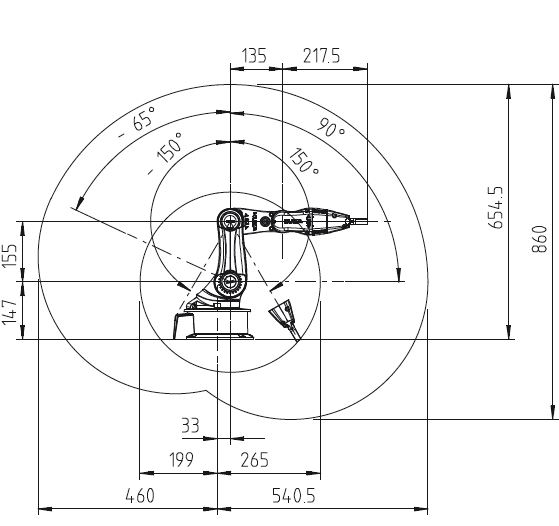
\includegraphics[width=0.7\textwidth]{youbot_workspace_1.jpg} \\ а)}
    \vfill
	\begin{minipage}[h]{0.47\linewidth}
		\centering{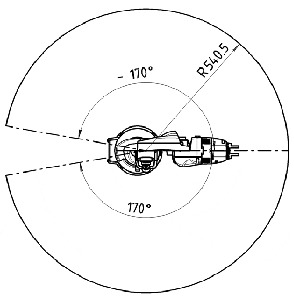
\includegraphics[width=0.95\linewidth]{youbot_workspace_2.jpg} \\ б)}
	\end{minipage}
	\hfill
	\begin{minipage}[h]{0.47\linewidth}
		\centering{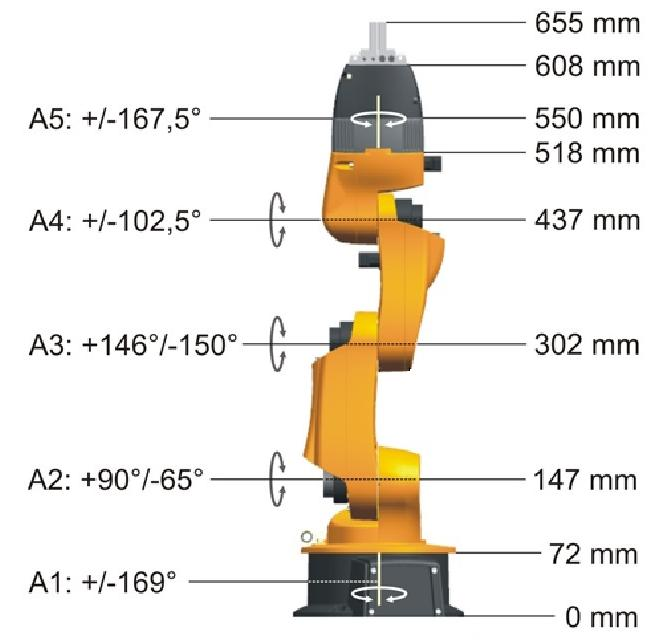
\includegraphics[width=0.95\linewidth]{youbot_length.jpg} \\ в)}
	\end{minipage}
	\caption{Некоторые параметры манипулятора Kuka Youbot: a~--- размеры рабочей области (вид сбоку); б~--- размеры рабочей области (вид сверху); в~--- длины звеньев и предельные значения для углов вращения по каждому из сочленений~\cite{youbot_detailed_specifications}.}
	\label{img:sizes_of_robot}
\end{figure}

\newpage
\section{Математическая модель манипулятора}\label{part_math_model_of_robot}
\subsection{Кинематика манипулятора}\label{part_kinematics}

\subsubsection{Общие замечания}

% TODO Тут обосновать зачем нужна кинематика манипулятора

Последовательная кинематическая цепь рассматриваемого манипулятора, включающая только вращательные КП V-класса (цилиндрические шарниры), изображена на рисунке~\ref{img:kinematics}a.

\begin{figure}[h!]
	\begin{minipage}[h]{0.5\linewidth}
		\centering{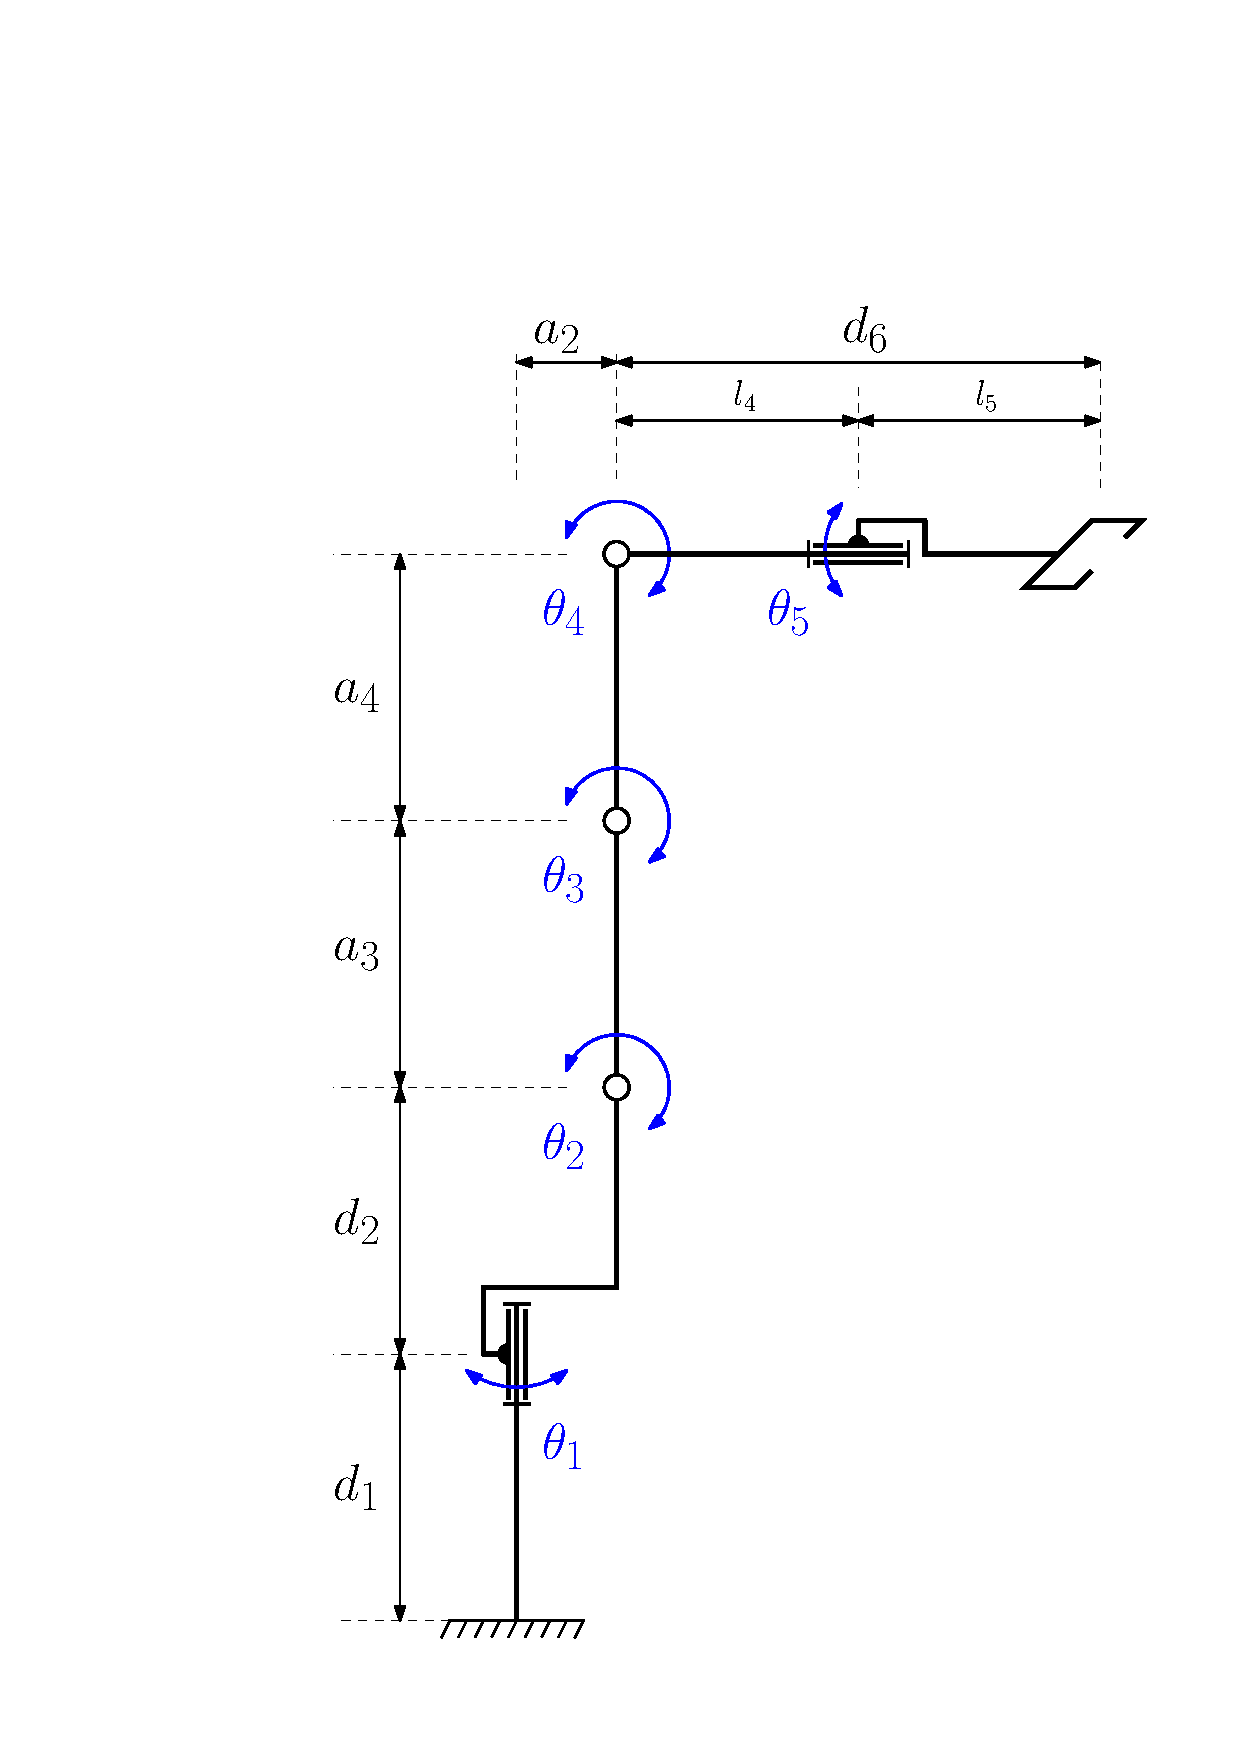
\includegraphics[width=0.95\linewidth]{kinematics_schema.pdf} \\ а)}
	\end{minipage}
	\hfill
	\begin{minipage}[h]{0.5\linewidth}
		\centering{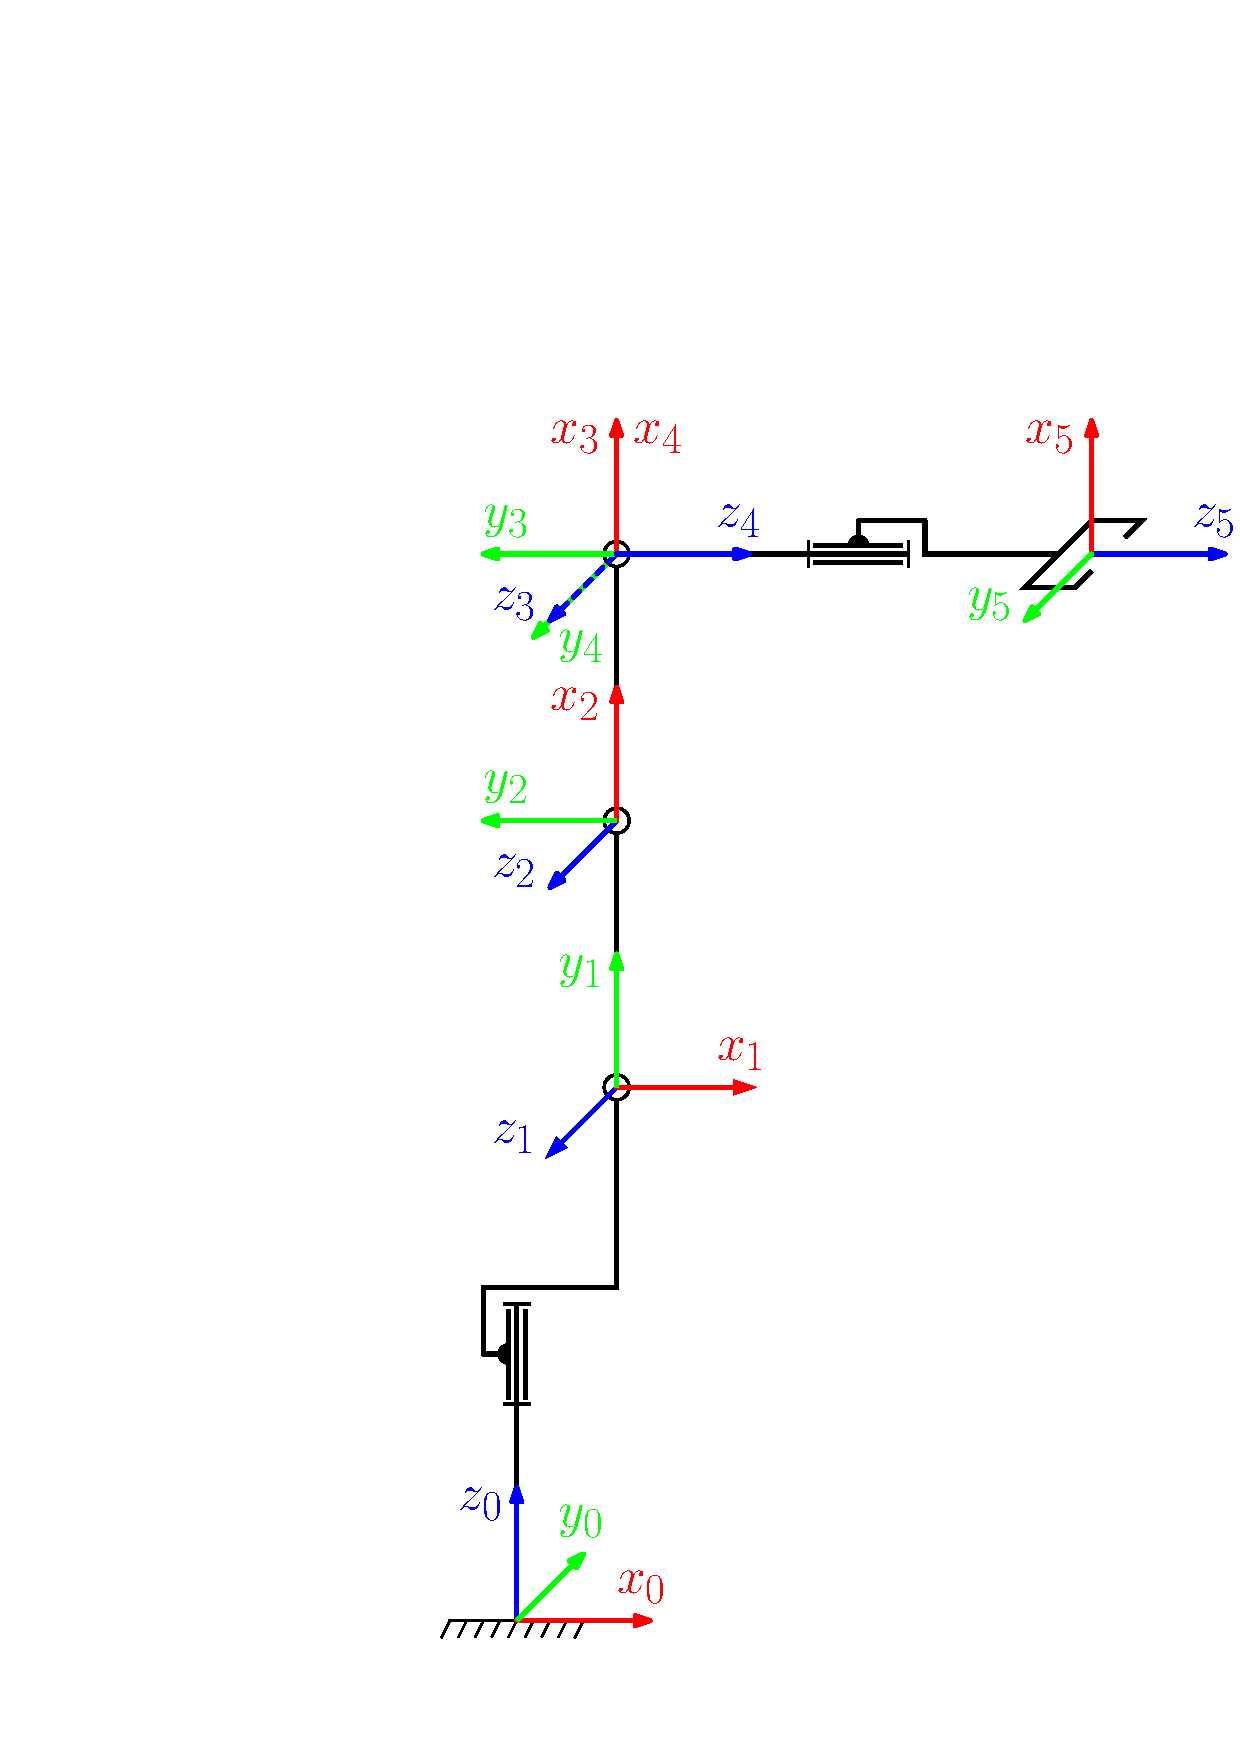
\includegraphics[width=0.95\linewidth]{kinematics_frames.pdf} \\ б)}
	\end{minipage}
	\caption{Схемы рассматриваемого манипулятора: а~--- кинематическая при $q_i=0$, $i=\overline{1,5}$; б~--- расположения СК КП.}
	\label{img:kinematics}
\end{figure}

Для описания положений звеньев манипулятора друг относительно друга воспользуемся методом Денавита--Хартенберга, состоящим из трех данных шагов:
\begin{enumerate}
    \item <<привязка>> к каждому звену СК, чьи оси удовлетворяют следующим условиям:
    \begin{enumerate}
	    \item ось $z_{i-1}$ направлена вдоль оси $i$-ой КП;
        \item ось $x_i$ перпендикулярна оси $z_{i-1}$ и пересекает ее;
        \item ось $y_i$ дополняет оси $z_i$ и $x_i$ до правой декартовой СК.
    \end{enumerate}
    \item определение параметров ДХ:
    \begin{enumerate}
	    \item $a_i$~--- расстояния от $z_{i-1}$ до $z_i$ вдоль $x_i$;
	    \item $\alpha_i$~--- угла от $z_{i-1}$ до $z_i$ вокруг $x_i$;
        \item $d_i$~--- расстояния от $x_{i-1}$ до $x_i$ вдоль $z_{i-1}$;
        \item $\theta_i$~--- угла от $x_{i-1}$ до $x_i$ вокруг $z_{i-1}$.
    \end{enumerate}
    \item расчет матриц однородного преобразования в соответствии со следующими формулами:
    \begin{equation}\label{DH_matrix}
        {}^{i-1}A_{i} = R_{z, \theta_i} \cdot T_{z, d_i} \cdot T_{x, a_i} \cdot R_{x, \alpha_i}
    \end{equation}
    где $R_{z, \theta_i}$~--- матрица поворота вокруг оси $z$ на угол $\theta_i$, $T_{z, d_i}$~--- матрица смещения вдоль оси $z$ на расстояние $d$, $T_{x, a_i}$~---матрица смещения вдоль оси $x$ на расстояние $a_i$,  $R_{x, \alpha_i}$~--- матрица поворота вокруг оси $x$ на угол $\alpha_i$, равные
    \begin{gather}
        R_{z, \theta_i} =
        \begin{bmatrix}
            \cos\theta_i & -\sin\theta_i & 0 & 0\\
            \sin\theta_i &  \cos\theta_i & 0 & 0\\
            0 & 0 & 1 & 0\\
            0 & 0 & 0 & 1
        \end{bmatrix}\!\!,
        \quad
        T_{z, d_i} =
        \begin{bmatrix}
            1 & 0 & 0 & 0\\
            0 & 1 & 0 & 0\\
            0 & 0 & 1 & d_i\\
            0 & 0 & 0 & 1\\
        \end{bmatrix}\!\!,\\
        %
        T_{x, a_i} =
        \begin{bmatrix}
            1 & 0 & 0 & a_i\\
            0 & 1 & 0 & 0\\
            0 & 0 & 1 & 0\\
            0 & 0 & 0 & 1\\
        \end{bmatrix}\!\!,
        \quad
        R_{x, \alpha_i} =
        \begin{bmatrix}
            1 & 0 & 0 & 0\\
            0 & \cos\alpha_i & -\sin\alpha_i & 0\\
            0 & \sin\alpha_i &  \cos\alpha_i & 0\\
            0 & 0 & 0 & 1
        \end{bmatrix}\!\!;
    \end{gather}
    итого
    \begin{equation}
        {}^{i-1}A_i =
        \begin{bmatrix}
            \cos\theta_i & - \cos\alpha_i \sin\theta_i & \sin\alpha_i \sin\theta_i & a_{i} \cos\theta_i\\
            \sin\theta_i & \cos\alpha_i \cos\theta_i & - \sin\alpha_i \cos\theta_i & a_{i} \sin\theta_i\\
            0 & \sin\alpha_i & \cos\alpha_i & d_{i}\\
            0 & 0 & 0 & 1
        \end{bmatrix}
    \end{equation}
\end{enumerate}

Результаты выполнения для исследуемого манипулятора двух первых шагов представлены на рисунке~\ref{img:kinematics}б и в таблице~\ref{table_DH_params}, а третьего~--- в лице следующих выражений:
\begin{gather}
	{}^0A_1\! =\!\!
    \left[\begin{matrix}c_1 & 0 & s_1 & a_{1} c_1\\s_1 & 0 & - c_1 & a_{1} s_1\\0 & 1 & 0 & d_{1}\\0 & 0 & 0 & 1\end{matrix}\right]\!\!;
    %
	{}^1A_2\! =\!\!
	\left[\begin{matrix}c_2 & - s_2 & 0 & a_{2} c_2\\s_2 & c_2 & 0 & a_{2} s_2\\0 & 0 & 1 & 0\\0 & 0 & 0 & 1\end{matrix}\right]\!\!;
    %
	{}^2A_3\! =\!\!
	\left[\begin{matrix}c_3 & - s_3 & 0 & a_{3} c_3\\s_3 & c_3 & 0 & a_{3} s_3\\0 & 0 & 1 & 0\\0 & 0 & 0 & 1\end{matrix}\right]\!\!;\notag
	\\
	{}^3A_4 =
	 \left[\begin{matrix}c_4 & 0 & s_4 & 0\\s_4 & 0 & - c_4 & 0\\0 & 1 & 0 & 0\\0 & 0 & 0 & 1\end{matrix}\right]\!\!;
	\;
	{}^4A_5 =
	\left[\begin{matrix}c_5 & - s_5 & 0 & 0\\s_5 & c_5 & 0 & 0\\0 & 0 & 1 & d_{5}\\0 & 0 & 0 & 1\end{matrix}\right]\!\!\ldotp
	\label{eq_all_ht_matrices}
\end{gather}

\begin{table}[h!]
	\caption{Параметры Денавита-Хартенберга}
	\begin{center}
		\begin{tabular}{|c|c|c|c|c|}
			\hline
			Звено 	& $a_i$, мм & $\alpha_i$, рад & $d_i$, мм & $\theta_i$, рад\\
			\hline
			1  		& $33$ & $\pi/2$ & $147$ & $q_1$\\
			\hline
			2 		& $155$ & $0$ 	& $0$ 	& $q_2 + \pi/2$\\
			\hline
			3 		& $135$ & $0$ 	& $0$ 	& $q_3$\\
			\hline
			4 		& $0$ & $\pi/2$ & $0$ 	& $q_4$\\
			\hline
			5 		& $0$ & $0$ 	& $218$ & $q_5$\\
			\hline
		\end{tabular}
	\end{center}
	\label{table_DH_params}
\end{table}


\subsubsection{Прямая задача кинематики}\label{part_kinematics_forward}
Информация о смещении и повороте СК $Ox_5y_5z_5$ относительно СК $Ox_0y_0z_0$ содержится в матрице ${}^0A_5$.
Следовательно, для того чтобы решить ПЗК, остается лишь найти эту матрицу в соответствии c формулой:
\begin{equation}\label{fk}
	{}^0A_5 = \prod^{5}_{i=1}{{}^{i-1}A_i(q_i)}\ldotp
\end{equation}

\begin{figure}[h]
	\centering
	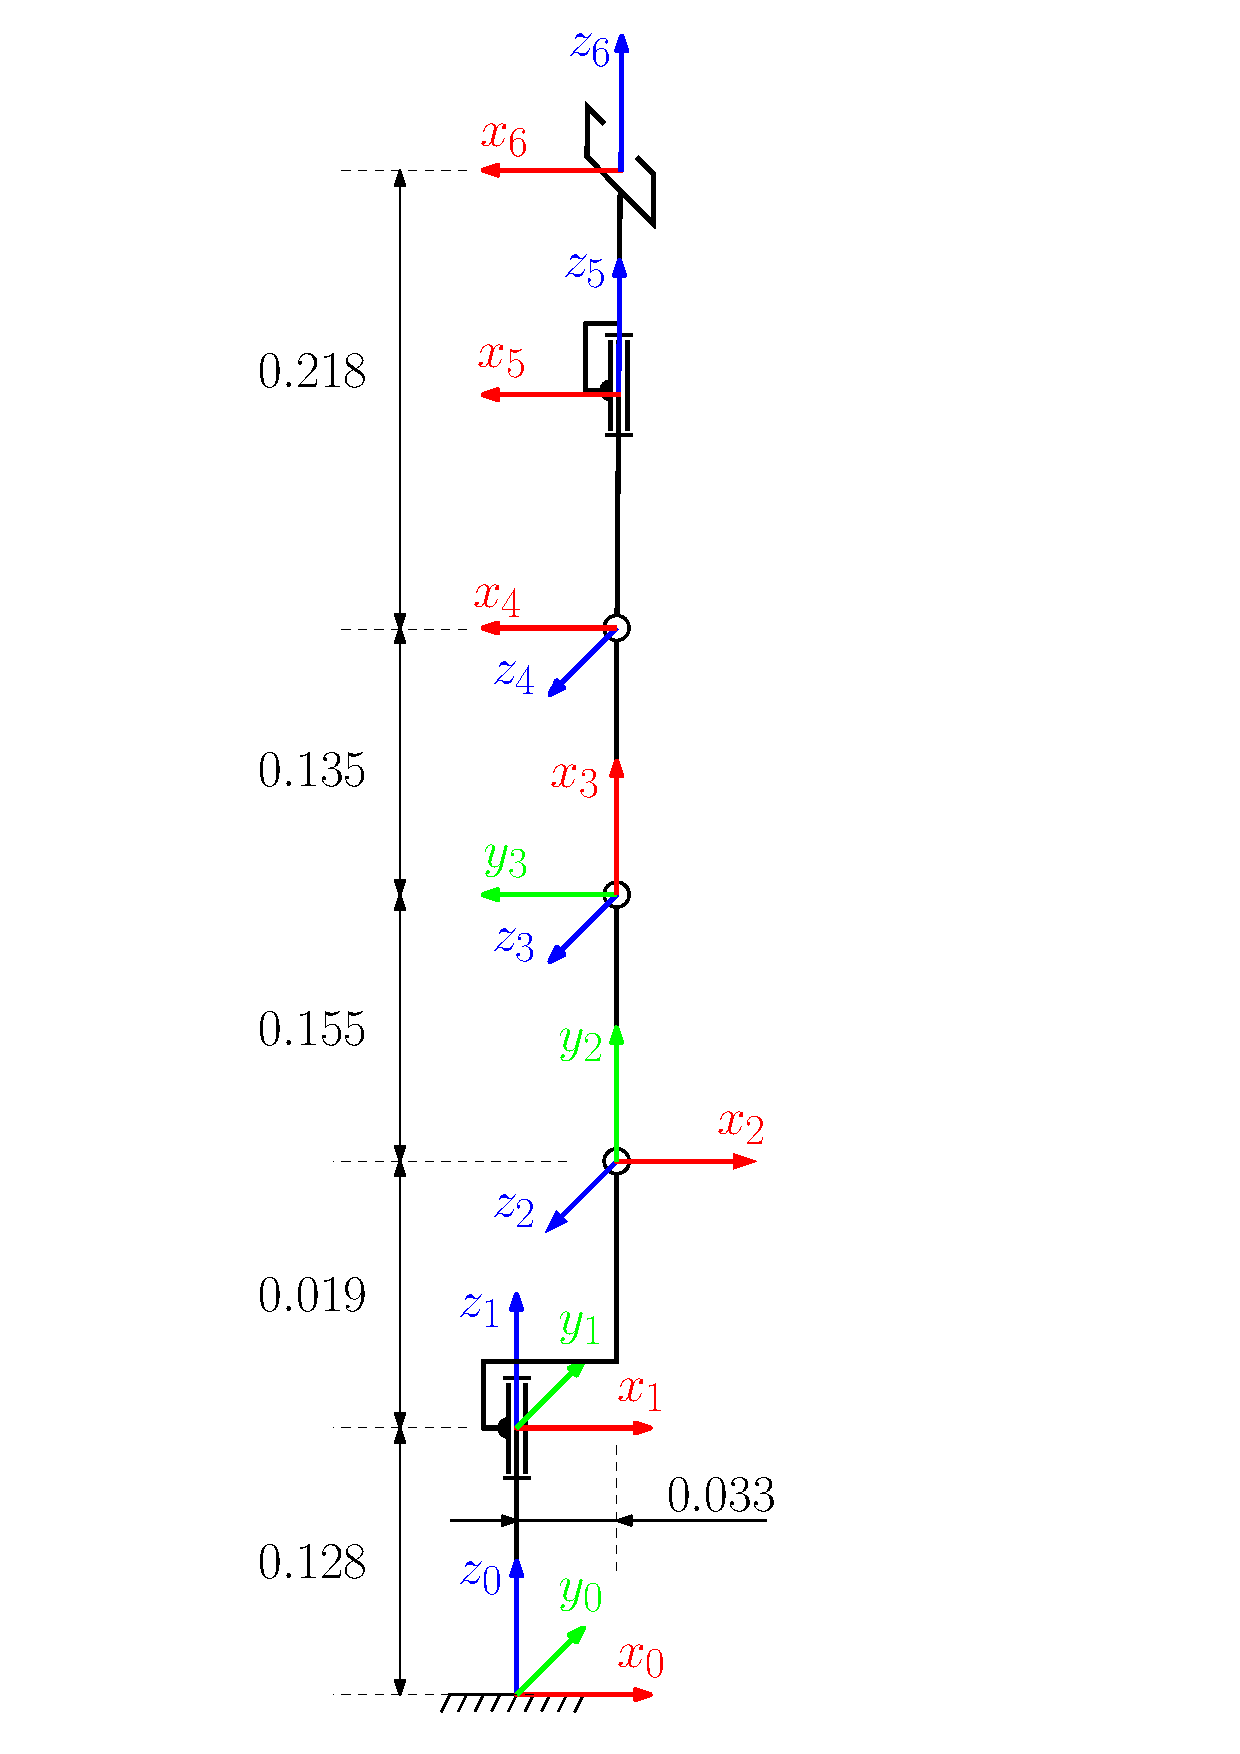
\includegraphics[width=0.2\textwidth]{kinematics_check.pdf}
	\caption{Конфигурация манипулятора при $q=\left[q_1,\,q_2,\,q_3,\,q_4,\,q_5\right] = \left[0,\,0,\,0,\,\pi/2,\,0\right]$.}
	\label{kinematics_check}
\end{figure}

Для проверки рассмотрим конфигурацию манипулятора, изображенную на рисунке~\ref{kinematics_check}.
В~результате решения для нее ПЗК должны получиться следующие матрица поворота и вектор смещения :
\begin{equation}
	{}^{0}R_5 =
	\begin{bmatrix}
		-1 &  0 & 0\\
		 0 & -1 & 0\\
		 0 &  0 & 1
	\end{bmatrix}\!\!,
	\qquad
	r^{0}_{0,\,5} =
	\begin{bmatrix}
		0.033\\
		0\\
		0.655
	\end{bmatrix}\!\!\ldotp
\end{equation}
Выполняя соответствующие вычисления получаем:
\begin{multline}
    {}^{0}A_5 = {}^{0}A_1 \cdot {}^{1}A_2 \cdot {}^{2}A_3 \cdot {}^{3}A_4 \cdot {}^{4}A_5 =
    \begin{bmatrix}
        1 & 0 &  0 & 0.033\\
        0 & 0 & -1 &     0\\
        0 & 1 &  0 & 0.147\\
        0 & 0 &  0 &     1
    \end{bmatrix}
    \cdot
    \begin{bmatrix}
        0 & -1 &  0 &     0\\
        1 &  0 &  0 & 0.155\\
        0 &  0 &  1 &     0\\
        0 &  0 &  0 &     1
    \end{bmatrix}
    \cdot \\ \cdot
    \begin{bmatrix}
        1 & 0 &  0 & 0.135\\
        0 & 1 &  0 &     0\\
        0 & 0 &  1 &     0\\
        0 & 0 &  0 &     1
    \end{bmatrix}
    \cdot
    \begin{bmatrix}
        0 & 0 & 1 & 0\\
        1 & 0 & 0 & 0\\
        0 & 1 & 0 & 0\\
        0 & 0 & 0 & 1
    \end{bmatrix}
    \cdot
     \begin{bmatrix}
        1 & 0 &  0 &     0\\
        0 & 1 &  0 &     0\\
        0 & 0 &  1 & 0.218\\
        0 & 0 &  0 &     1
    \end{bmatrix}
    =
    \left[\begin{matrix}-1 & 0 & 0 & 0.033\\0 & -1 & 0 & 0\\0 & 0 & 1 & 0.655\\0 & 0 & 0 & 1\end{matrix}\right]\!\!,
\end{multline}
что предложенный способ решения ПЗК в данном случае приводит к правильному ответу.

\subsubsection{Обратная задача кинематики}\label{part_kinematics_inverse}
Заданные смещение и поворот СК $Ox_5y_5z_5$ относительно СК $Ox_0y_0z_0$ можно описать с помощью матрицы ${}^0A_5$.
Используя ее и матрицы из~\eqref{eq_all_ht_matrices}, найти расчетные формулы для углов $q_i$ ($i=\overline{1,5}$) можно из следующих соображений.

Введем обозначения для элементов матрицы ${}^0A_5$ в соответствии с формулой:
\begin{equation}\label{ik}
	{}^0A_5 =
	\left[\begin{matrix}
	r_{11} & r_{12} & r_{13} & p_{x}\\
	r_{21} & r_{22} & r_{23} & p_{y}\\
	r_{31} & r_{32} & r_{33} & p_{z}\\
	0 & 0 & 0 & 1
	\end{matrix}\right]\!\!\ldotp
\end{equation}

Приравняв матрицу ${}^0A_5$ и правую часть выражения~\eqref{fk} и домножив с обеих сторон на ${}^0A_1^{-1}$, придем к выражению:
\begin{equation}
	{}^0A_1^{-1} \cdot {}^0A_5 = {}^1A_2 \cdot {}^2A_3 \cdot {}^3A_4 \cdot {}^4A_5,
\end{equation}
где левая часть с учетом~\eqref{eq_all_ht_matrices} равна
\begin{equation}\label{eq_left_part}
	{}^0A_1^{-1} \cdot {}^0A_5 =
	\left[\begin{matrix}
		r_{11} c_{1} + r_{21} s_{1} & r_{12} c_{1} + r_{22} s_{1} & r_{13} c_{1} + r_{23} s_{1} &  p_{x} c_{1} + p_{y} s_{1} - a_{1}\\
		r_{31} & r_{32} & r_{33} & p_{z} - d_{1}\\
		r_{11} s_{1} - r_{21} c_{1} & r_{12} s_{1} - r_{22} c_{1} & r_{13} s_{1} - r_{23} c_{1} & p_{x} s_{1} - p_{y} c_{1}\\
		0 & 0 & 0 & 1\end{matrix}\right]\!\!,
\end{equation}
а правая~---
\begin{equation}\label{eq_right_part}
	{}^1A_2 \cdot {}^2A_3 \cdot {}^3A_4 \cdot {}^4A_5 =
	\left[\begin{matrix}
		c_{5} c_{234} & - s_{5} c_{234} & s_{234} & a_{2} c_{2} + a_{3} c_{23} + d_{5} s_{234}\\
		c_{5} s_{234} & - s_{5} s_{234} & - c_{234} & a_{2} s_{2} + a_{3} s_{23} - d_{5} c_{234}\\
		s_{5} & c_{5} & 0 & 0\\
		0 & 0 & 0 & 1
	\end{matrix}\right]\!\!,
\end{equation}
где в свою очередь
\begin{equation}\label{eq_theta_23_234}
    \theta_{23} = \theta_2 + \theta_3,
    \qquad
    \theta_{234} = \theta_2 + \theta_3 + \theta_4\ldotp
\end{equation}

Теперь, сопоставляя элементы матриц с одинаковыми индексами из выражений~\eqref{eq_left_part} и \eqref{eq_right_part}, получим, что расчетные формулы для двух наборов значений углов $\theta_1$, $\theta_5$ и $\theta_{234}$ дают
\begin{itemize}
    \item равенство элементов $(3,4)$:
        \begin{equation}\label{eq_for_theta_1}
	        p_{x} s_{1} - p_{y} c_{1} = 0
            \; \Rightarrow \;
	        \tg \theta_1 = \cfrac{p_y}{p_x}
	        \; \Rightarrow \;
	        \left\{
	        \begin{aligned}
		        \!&\theta_1^\msf{I} = \atan2(p_y, p_x)\\
		        \!&\theta_1^\msf{II} = \atan2(-p_y, -p_x)
            \end{aligned}
            \right.
        \end{equation}
    \item равенство элементов $(3,1)$ и $(3,2)$:
        \begin{multline}
            \left\{
	        \begin{aligned}
		        \!&s_{5} = r_{11} s_{1} - r_{21} c_{1}\\
		        \!&c_{5} = r_{12} s_{1} - r_{22} c_{1}
            \end{aligned}
            \right.
            \qquad \Rightarrow
            \\
            \Rightarrow \;
            \left\{
	        \begin{aligned}
		        \!&\theta_5^\msf{I} = \atan2(r_{11} \sin\theta_1^\msf{I} - r_{21} \cos\theta_1^\msf{I},\: r_{12} \sin\theta_1^\msf{I} - r_{22} \cos\theta_1^\msf{I})\\
		        \!&\theta_5^\msf{II} = \atan2(r_{11} \sin\theta_1^\msf{II} - r_{21} \cos\theta_1^\msf{II},\: r_{12} \sin\theta_1^\msf{II} - r_{22} \cos\theta_1^\msf{II})
            \end{aligned}
            \right.
        \end{multline}
    \item равенство элементов $(2,3)$ и $(1,3)$:
        \begin{multline}
            \left\{
	        \begin{aligned}
		        \!&c_{234} = -r_{33}\\
		        \!&s_{234} = r_{13} c_{1} + r_{23} s_{1}
            \end{aligned}
            \right.
            \qquad \Rightarrow
            \\
            \Rightarrow \qquad
            \left\{
	        \begin{aligned}
		        \!&\theta_{234}^\msf{I} = \atan2(r_{13} \cos\theta_1^\msf{I}  + r_{23} \sin\theta_1^\msf{I},\: -r_{33})\\
		        \!&\theta_{234}^\msf{II} = \atan2(r_{13} \cos\theta_1^\msf{II}  + r_{23} \sin\theta_1^\msf{II},\: -r_{33})
            \end{aligned}
            \right.
        \end{multline}
\end{itemize}

Далее домножим выражение~\eqref{eq_left_part} на ${}^4A_5^{-1}$ справа~--- получим матрицу~${}^1A_4$:
\begin{equation}\label{eq_A14_matrix}
    {}^1A_4 =
    \begin{bmatrix}
        \cdots & \cdots & \cdots & (p_y - d_5 r_{23})s_1 + (p_x - d_5 r_{13})c_1 - a_1\\
        \cdots & \cdots & \cdots & p_z - d_1 - d_5 r_{33}\\
        \cdots & \cdots & \cdots & p_x s_1 - p_y c_1 - d_5(r_{13} s_1 - r_{23} c_1)\\
        0 & 0 & 0 & 1
    \end{bmatrix}\!\!,
\end{equation}
в которой символами $\cdots$ обозначены элементы, не представляющие интереса в дальнейших расчетах.
Заметим, что c учетом~\eqref{eq_for_theta_1} и равенства элементов~$(3,3)$ в~\eqref{eq_left_part} и~\eqref{eq_right_part} справедливо
\begin{equation}
p_x s_1 - p_y c_1 - d_5(r_{13} s_1 - r_{23} c_1) = 0\ldotp
\end{equation}
С~учетом этого и~\eqref{eq_A14_matrix}, имеем что
\begin{equation}\label{eq_r_1_1_4}
    r^1_{1,\,4} =
    \begin{bmatrix}
        (p_y - d_5 r_{23})s_1 + (p_x - d_5 r_{13})c_1 - a_1 \\
        p_z - d_1 - d_5 r_{33} \\
        0
    \end{bmatrix}\!\!\ldotp
\end{equation}

Далее заметим, что одно и то же положение 4-го звена может достигаться при двух разных способах расположения звеньев~2 и~3 (см.~рисунок~\ref{ik_geometric}).
Следовательно, углы $\theta_2$, $\theta_3$ и $\theta_4$ при одних и тех же значениях углов $\theta_1$ и $\theta_5$ имеют по два возможных значения.
Ниже выводятся формулы для последних.

\begin{figure}[h!]
	\centering
	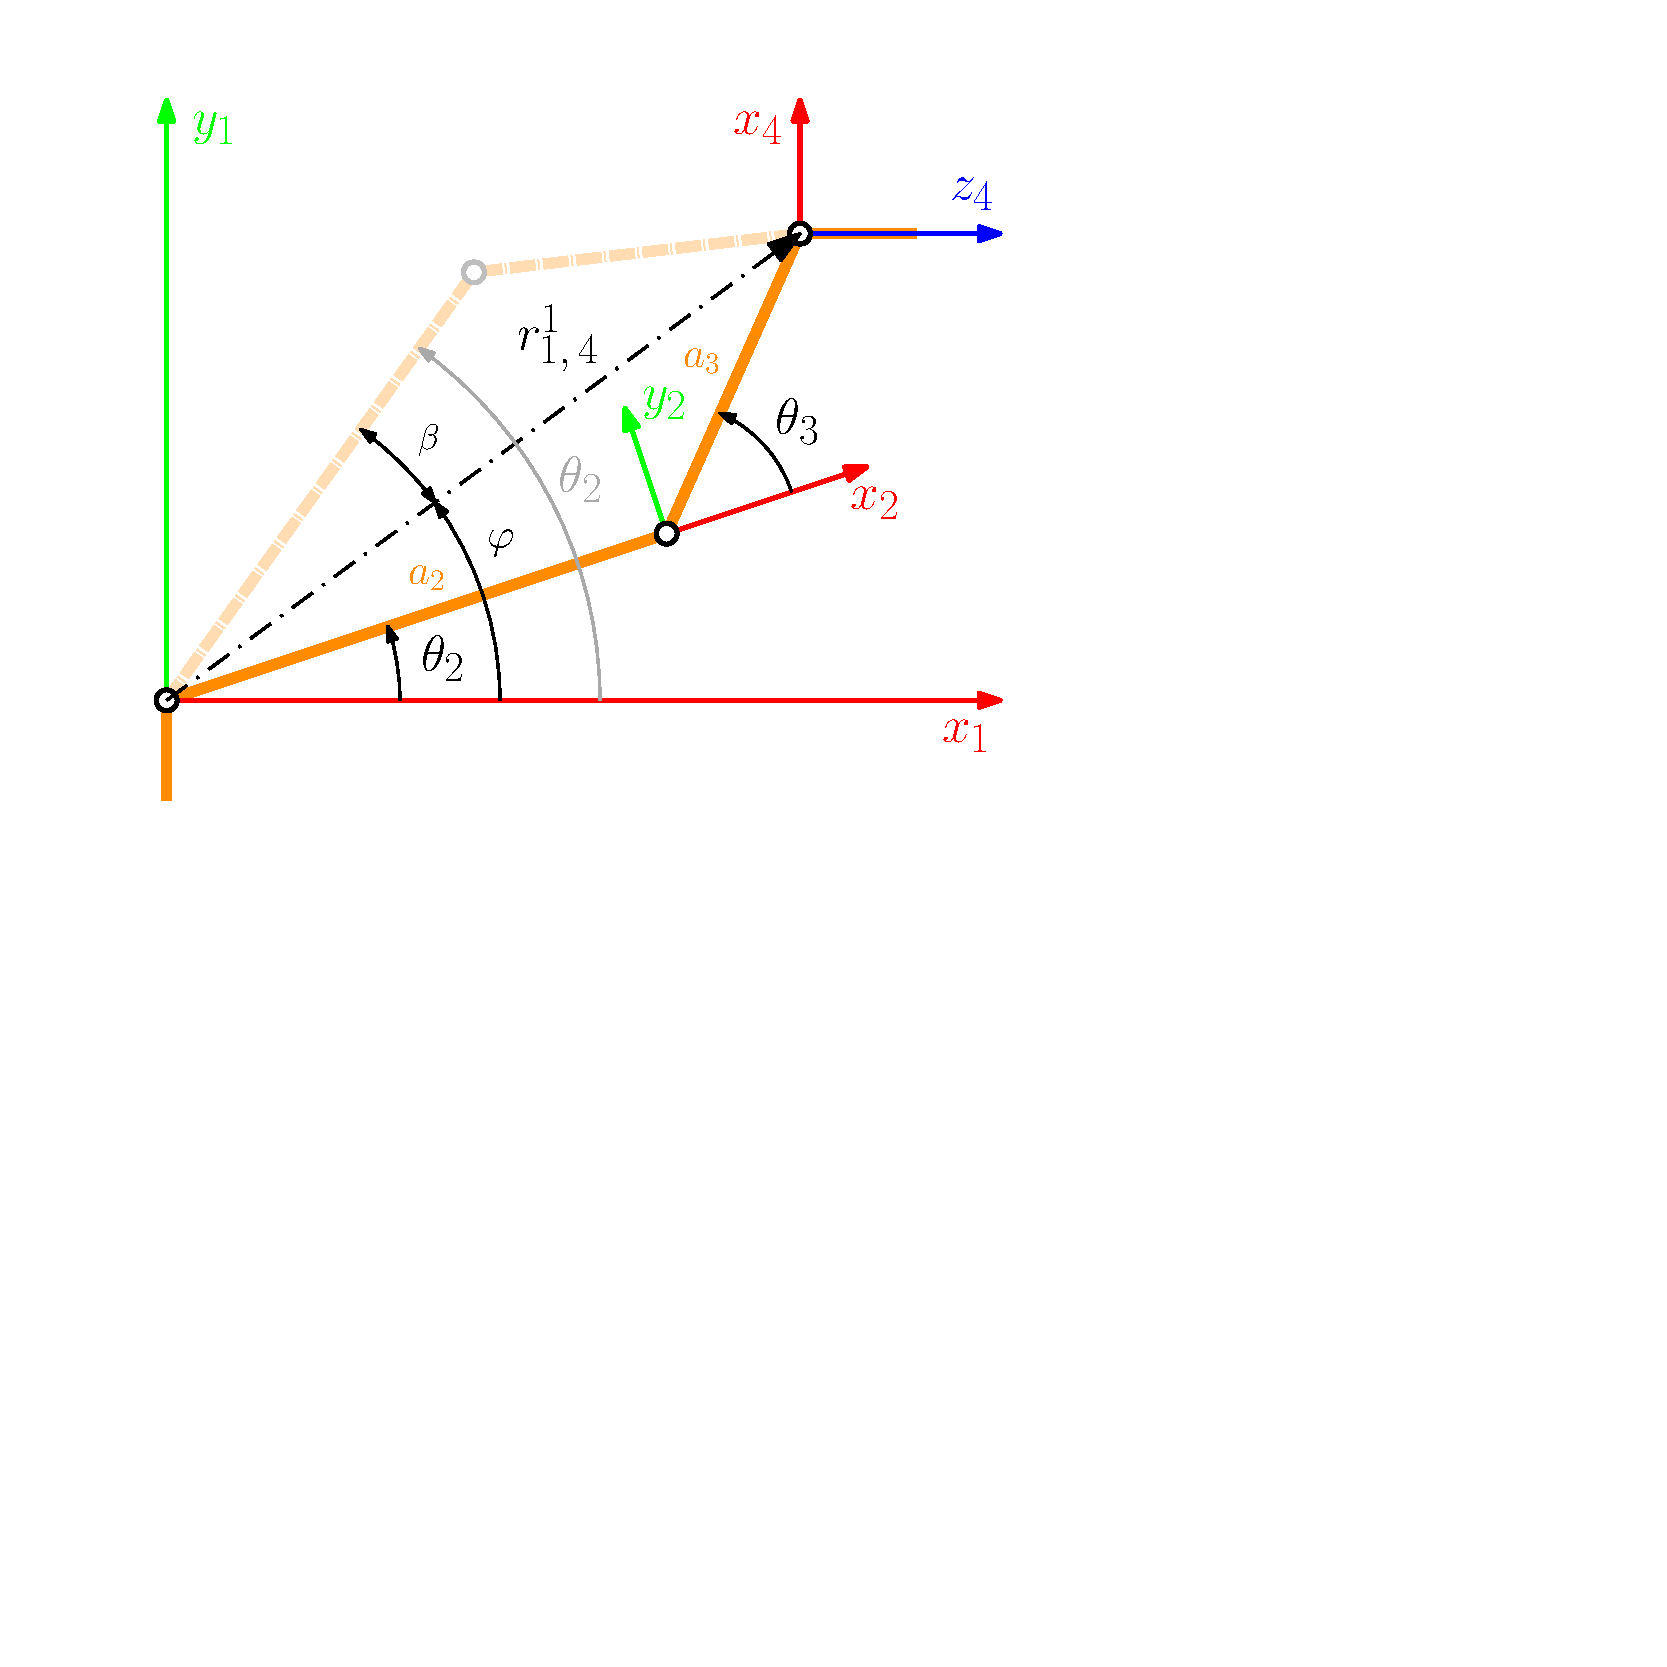
\includegraphics[width=0.7\textwidth]{ik_geometric_approach.pdf}
	\caption{Плоская часть манипулятора}
	\label{ik_geometric}
\end{figure}

Выпишем, пользуясь теоремой косинусов, выражение для $\cos\theta_3$ (его зависимость от $\theta_1$ обуславливается зависимостью от этого угла вектора $r^1_{1,\,4}$):
\begin{equation}
	c_3(\theta_1) = \frac{(r^1_{1,\,4})^T \!\! \cdot r^1_{1,\,4}- a_2^2 - a_3^2}{2 a_2 a_3}
\end{equation}
C~учетом этого для $\theta_3$ можно получить следующие формулы
\begin{gather}
	\theta_3^\msf{I,II} = \mp \atan2\bigl(\sqrt{1 - c_3^2(\theta_1^\msf{I})},\; c_3(\theta_1^\msf{I})\bigr)\\
	\theta_3^\msf{III,IV} = \mp \atan2\bigl(\sqrt{1 - c_3^2(\theta_1^\msf{II})},\; c_3(\theta_1^\msf{II})\bigr)
\end{gather}

Как видно из рисунка~\ref{ik_geometric}, $\theta_2 = \varphi + \beta$ при $\theta_3^\msf{I,III} < 0$ и $\theta_2 = \varphi - \beta$ при $\theta_3^\msf{II,IV} > 0$.
Следовательно, принимая во внимание то, что
\begin{equation}
    \varphi(\theta_1) = \atan2(y_r,\, x_r),
    \qquad
    \beta(\theta_3) = \atan2(a_3\sin|\theta_3|,\: a_2 + a_3\cos|\theta_3|),
\end{equation}
где $x_r$ и $y_r$~--- проекции вектора $r^1_{1,\,4}$ на оси абсцисс и ординат (их значения см.~в~\eqref{eq_r_1_1_4}), для возможных значений угла $\theta_2$ получаем следующие формулы:
\begin{align}
	\theta_2^\msf{I} &= \varphi(\theta_1^\msf{I}) + \beta(\theta_3^\msf{I}), &
	\theta_2^\msf{II} &= \varphi(\theta_1^\msf{I}) - \beta(\theta_3^\msf{II}),\\
	\theta_2^\msf{III} &= \varphi(\theta_1^\msf{II}) + \beta(\theta_3^\msf{III}), &
	\theta_2^\msf{IV} &= \varphi(\theta_1^\msf{II}) - \beta(\theta_3^\msf{IV})\ldotp
\end{align}

Формулы для значений угла $\theta_4$ после этого с учетом~\eqref{eq_theta_23_234} приобретают простой вид:
\begin{equation}
	\theta_4^\msf{I,II} = \theta_{234}^\msf{I} - \theta_{2}^\msf{I,II} - \theta_{3}^\msf{I,II},
	\qquad
	\theta_4^\msf{III,IV} = \theta_{234}^\msf{II} - \theta_{2}^\msf{III, IV} - \theta_{3}^\msf{III,IV}\ldotp
\end{equation}

Таким образом, любые положение и ориентацию схвата относительно основания манипулятор может обеспечить 4-мя собственными конфигурациями, которым соответствуют следующие наборы значений для его обобщенных координат $q=\left[q_1,\,q_2,\,q_3,\,q_4,\,q_5\right]$ (с~учетом таблицы~\ref{table_DH_params}):
\begin{align}
	q^\msf{I} &=
	\begin{bmatrix}
	    \theta_1^\msf{I} & \theta_2^\msf{I} - \cfrac{\pi}{2} & \theta_3^\msf{I} & \theta_4^\msf{I} & \theta_5^\msf{I}
	\end{bmatrix}\!\!,
	&
	q^\msf{II} &=
	\begin{bmatrix}
	    \theta_1^\msf{I} & \theta_2^\msf{II} - \cfrac{\pi}{2} & \theta_3^\msf{II} & \theta_4^\msf{II} & \theta_5^\msf{I}
	\end{bmatrix}\!\!,
	\\
	q^\msf{III} &=
	\begin{bmatrix}
	    \theta_1^\msf{II} & \theta_2^\msf{III} - \cfrac{\pi}{2} & \theta_3^\msf{III} & \theta_4^\msf{III} & \theta_5^\msf{II}
	\end{bmatrix}\!\!,
	&
	q^\msf{IV} &=
	\begin{bmatrix}
	    \theta_1^\msf{II} & \theta_2^\msf{IV} - \cfrac{\pi}{2} & \theta_3^\msf{IV} & \theta_4^\msf{IV} & \theta_5^\msf{II}
	\end{bmatrix}\!\!\ldotp
\end{align}

\newpage

\subsection{Динамика манипулятора}\label{part_dynamics}

\subsubsection{Общие замечания}
Введем в рассмотрение барицентрические СК $Ox_{ci}y_{ci}z_{ci}$\lefteqn,\footnote{Системы координат, чьи начала совпадают с центрами масс соответствующих звеньев.} где $i=\overline{1,5}$, показанные на рисунке~\ref{img_mass_frames}.
Заметим, что каждая СК $Ox_{ci}y_{ci}z_{ci}$ сонаправлена с~$Ox_iy_iz_i$.

\begin{figure}[h!]
	\centering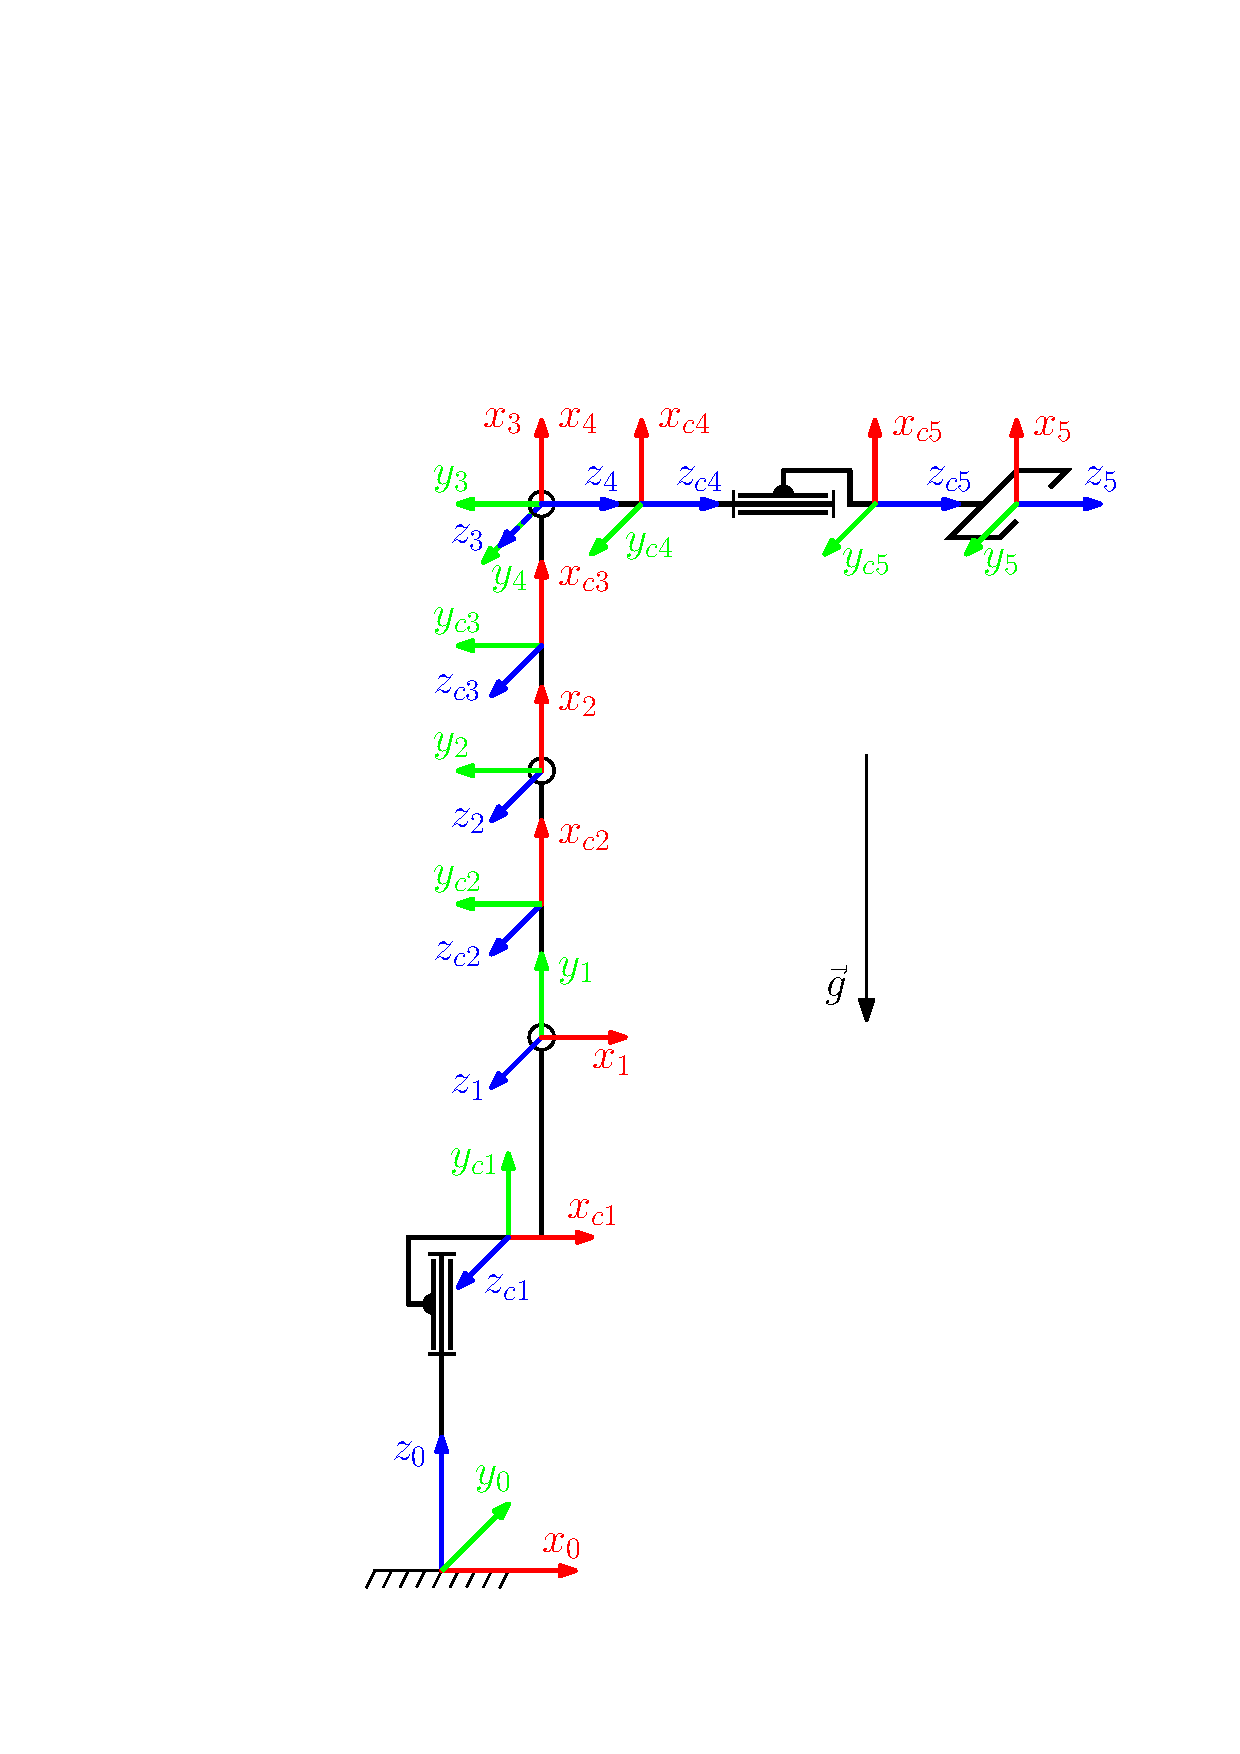
\includegraphics[height=16.5cm]{kinematics_mass_frames.pdf}
	\caption{Положение барицентрических СК и направление вектора $\vec{g}$.}
	\label{img_mass_frames}
\end{figure}

Для описания положения введенных СК воспользуемся следующими векторами:
\begin{equation}
    r^i_{i,\,ci} =
    \begin{bmatrix}
        x_{ci} \\ y_{ci} \\ z_{ci}
    \end{bmatrix}\!\!,\quad i = \overline{1,5},
\end{equation}
где $x_{ci}$, $y_{ci}$ и $z_{ci}$~--- некоторые постоянные величины.

Для компонент тензоров инерции $\mathcal{I}^{i}_i = const$ введем следующие обозначения:
\begin{equation}
    \mathcal{I}^{i}_i =
    \begin{bmatrix}
        I_{i,\,xx} & I_{i,\,xy} & I_{i,\,xz} \\
        I_{i,\,xy} & I_{i,\,yy} & I_{i,\,yz} \\
        I_{i,\,xz} & I_{i,\,yz} & I_{i,\,zz}
    \end{bmatrix}\!\!\ldotp
\end{equation}

Заметим, что
\begin{equation}
    g_0 =
    \begin{bmatrix}
        0 \\ 0 \\ -g
    \end{bmatrix}\!\!,
\end{equation}
где $g=9.82\text{ м}/\text{с}^2$.

В~заключении раздела приведем формулы для расчета величин, которые потребуются в дальнейшем (везде $i = \overline{1,5}$):
\begin{itemize}
    \item для расчета $r^0_{0,\,i}$ и ${}^{0}R_i$ (см.~Приложение~\ref{app_ht_matrices}):
        \begin{equation}
            {}^0A_i = {}^0A_1 \cdot {}^1A_2 \cdot \ldots \cdot {}^{i-1}A_i;
        \end{equation}
    \item для расчета $r^i_{0,\,i}$:
        \begin{gather}
            r^i_{0,\,i} = {}^{0}R_i^T \cdot r^0_{0,\,i};
        \end{gather}
    \item для расчета $z^0_i$:
        \begin{equation}
            z^0_i = {}^{0}R_i \cdot z^i_i = {}^{0}R_i \cdot
            \begin{bmatrix}
                0 \\ 0 \\ 1
            \end{bmatrix}\!\!;
        \end{equation}
    \item для расчета $g_i$, $v^i_i$ и $\omega^i_i$:
        \begin{equation}\label{eq_transform_of_g_v_omega}
            g_i = {}^{0}R_i^T \cdot g_0,
            \qquad
            v^i_i = {}^{0}R_i^T \cdot v^0_i,
            \qquad
            \omega^i_i = {}^{0}R_i^T \cdot \omega^0_i \ldotp
        \end{equation}
\end{itemize}

\subsubsection{Вывод уравнений движения}
Потенциальная энергия манипулятора
\begin{equation}
    U =  -\sum_{i=1}^5 \left( m_i g_i^T r^i_{0,\,ci} \right) = -\sum_{i=1}^5 \left( m_i g_i^T r^i_{0,\,i} + g_i^T (m_ir^i_{i,\,ci}) \right)\!,
\end{equation}


Якобианы, устанавливающие в соответствии с формулой
\begin{equation}\label{eq_work_of_lin_jacobians}
    v^0_{i} = J_{vi}\dot{q}, \quad i = \overline{1,5}
\end{equation}
связь между линейными скоростями начал соответствующих СК и вектором~$\dot{q}$:
\begin{gather}
    J_{v1} =
    \begin{bmatrix}
        z^0_0 \times \left( r^0_{0,\,1} - r^0_{0,\,0}\right) & \nv & \nv & \nv & \nv
    \end{bmatrix}\!\!,
    \\
    J_{v2} =
    \begin{bmatrix}
        z^0_0 \times \left( r^0_{0,\,2} - r^0_{0,\,0}\right) & z^0_1 \times \left( r^0_{0,\,2} - r^0_{0,\,1}\right) & \nv & \nv & \nv
    \end{bmatrix}\!\!,
    \\
    J_{v3} =
    \begin{bmatrix}
        z^0_0 \times \left( r^0_{0,\,3} - r^0_{0,\,0}\right) & z^0_1 \times \left( r^0_{0,\,3} - r^0_{0,\,1}\right) &
        z^0_2 \times \left( r^0_{0,\,3} - r^0_{0,\,2}\right) & \nv & \nv
    \end{bmatrix}\!\!,
    \\
    J_{v4} =
    \begin{bmatrix}
        z^0_0 \times \left( r^0_{0,\,4} - r^0_{0,\,0}\right) \\
        z^0_1 \times \left( r^0_{0,\,4} - r^0_{0,\,1}\right) \\
        z^0_2 \times \left( r^0_{0,\,4} - r^0_{0,\,2}\right) \\
        z^0_3 \times \left( r^0_{0,\,4} - r^0_{0,\,3}\right) \\
        \nv
    \end{bmatrix}^T\!\!\!\!\!,
    \qquad
    J_{v5} =
    \begin{bmatrix}
        z^0_0 \times \left( r^0_{0,\,5} - r^0_{0,\,0}\right) \\
        z^0_1 \times \left( r^0_{0,\,5} - r^0_{0,\,1}\right) \\
        z^0_2 \times \left( r^0_{0,\,5} - r^0_{0,\,2}\right) \\
        z^0_3 \times \left( r^0_{0,\,5} - r^0_{0,\,3}\right) \\
        z^0_4 \times \left( r^0_{0,\,5} - r^0_{0,\,4}\right)
    \end{bmatrix}^T\!\!\!\!\!,
\end{gather}
где $\nv = [0\;0\;0]^T$~--- нулевой вектор.

Якобианы, устанавливающие в соответствии с формулой
\begin{equation}\label{eq_work_of_ang_jacobians}
    \omega^0_{i} = J_{\omega i}\dot{q}, \quad i = \overline{1,5}
\end{equation}
связь между угловыми скоростями звеньев и вектором~$\dot{q}$:
\begin{gather}
    J_{\omega 1} =
    \begin{bmatrix}
        z^0_0 & \nv & \nv & \nv & \nv
    \end{bmatrix}\!\!,
    \qquad
    J_{\omega 2} =
    \begin{bmatrix}
        z^0_0 & z^0_1 & \nv & \nv & \nv
    \end{bmatrix}\!\!,
    \\
    J_{\omega 3} =
    \begin{bmatrix}
         z^0_0 & z^0_1 & z^0_2 & \nv & \nv
    \end{bmatrix}\!\!,
    \qquad
    J_{\omega 4} =
    \begin{bmatrix}
        z^0_0 & z^0_1 & z^0_2 & z^0_3 & \nv
    \end{bmatrix}\!\!,
    \\
    J_{\omega 5} =
    \begin{bmatrix}
        z^0_0 & z^0_1 & z^0_2 & z^0_3 & z^0_4
    \end{bmatrix}\!\!\ldotp
\end{gather}

Кинетическая энергия манипулятора
\begin{equation}\label{eq_eq_for_K_for_linear_model}
    K = \sum_{i=1}^5 \left( \frac{1}{2} m_i (v^i_i)^T v^i_i + \frac{1}{2} (\omega^i_i)^T \mathcal{I}^{i}_i \omega^i_i + (m_ir^i_{i,\,ci})^T \cdot (v^i_i \times \omega^i_i) \right)  \ldotp
\end{equation}

Функция Лагранжа
\begin{gather}
    L = K - U = \notag
    \\
    = \sum_{i=1}^5 \Biggl( m_i \left( \frac{1}{2} (v^i_i)^T v^i_i + g_i^T r^i_{0,\,i} \right) + (m_ir^i_{i,\,ci})^T \cdot \left( v^i_i \times \omega^i_i + g_i \right) + \frac{1}{2} (\omega^i_i)^T \mathcal{I}^{i}_i \omega^i_i \Biggr) = \notag
    \\
    = \sum_{i=1}^5 \Biggl( m_i \underbrace{\left( \frac{1}{2} (v^i_i)^T v^i_i + g_i^T r^i_{0,\,i} \right)}_{\ds L_{i,1}} + m_i x_{ci} \cdot \underbrace{x\left\{ v^i_i \times \omega^i_i + g_i \right\}}_{\ds L_{i,2}} + \notag
    \\
    + m_i y_{ci} \cdot \underbrace{y\left\{ v^i_i \times \omega^i_i + g_i \right\}}_{\ds L_{i,3}} + m_i z_{ci} \cdot \underbrace{z\left\{ v^i_i \times \omega^i_i + g_i \right\}}_{\ds L_{i,4}} + I_{i,\,xx} \cdot \underbrace{\frac{1}{2} \cdot \bigl(x\{\omega^i_i\}\bigr)^2}_{\ds L_{i,5}} +\notag
    \\
    + I_{i,\,yy} \cdot \underbrace{\frac{1}{2} \cdot \bigl(y\{\omega^i_i\}\bigr)^2}_{\ds L_{i,6}} + I_{i,\,zz} \cdot \underbrace{\frac{1}{2} \cdot \bigl(z\{\omega^i_i\}\bigr)^2}_{\ds L_{i,7}} + I_{i,\,xy} \cdot \underbrace{x\{\omega^i_i\} \cdot y\{\omega^i_i\}}_{\ds L_{i,8}} +\notag
    \\
    + I_{i,\,xz} \cdot \underbrace{x\{\omega^i_i\} \cdot z\{\omega^i_i\}}_{\ds L_{i,9}} + I_{i,\,yz} \cdot \underbrace{y\{\omega^i_i\} \cdot z\{\omega^i_i\}}_{\ds L_{i,10}}\Biggr) \ldotp
\end{gather}

Уравнения движения робота:
\begin{equation}
    \frac{d}{dt}\frac{\partial L}{\partial\dot{q_i}} - \frac{\partial L}{\partial q_i} = \tau_i, \quad i = \overline{1,5} \qquad \Rightarrow
\end{equation}
\begin{equation}
    \Rightarrow \quad
	\left\{
	\begin{aligned}
		\!&\sum_{i=1}^5 \bigl( m_i \cdot \mathcal{L}_1 \{L_{i,1}\} + m_i x_{ci} \cdot \mathcal{L}_1 \{L_{i,2}\} + \ldots + I_{i,\,yz} \cdot \mathcal{L}_1 \{L_{i,10}\} \bigr) = \tau_1\\
		\!&\sum_{i=1}^5 \bigl( m_i \cdot \mathcal{L}_2 \{L_{i,1}\} + m_i x_{ci} \cdot \mathcal{L}_2 \{L_{i,2}\} + \ldots + I_{i,\,yz} \cdot \mathcal{L}_2 \{L_{i,10}\} \bigr) = \tau_2\\
		\!&\ldots\\
		\!&\sum_{i=1}^5 \bigl( m_i \cdot \mathcal{L}_5 \{L_{i,1}\} + m_i x_{ci} \cdot \mathcal{L}_5 \{L_{i,2}\} + \ldots + I_{i,\,yz} \cdot \mathcal{L}_5 \{L_{i,10}\} \bigr) = \tau_5
	\end{aligned}
	\right.
\end{equation}
где $\mathcal{L}_j$~--- оператор, работающий в соответствии с формулой:
\begin{equation}
    \mathcal{L}_j : \quad \mathcal{L}_j \{f\} = \frac{d}{dt}\frac{\partial f}{\partial\dot{q_j}} - \frac{\partial f}{\partial q_j},
\end{equation}
где в свою очередь $f = f(\dot{q}(t), q(t))$.
Если же заметить, что
\begin{equation}
    \mathcal{L}_j \{L_{i,k}\} = 0 \qquad \text{при }j > i, \quad i,j=\overline{1,5}, \quad k=\overline{1,10},
\end{equation}
то выражения для них упрощаются до:
\begin{equation}
	\left\{
	\begin{aligned}
		\!&\sum_{i=1}^5 \bigl( m_i \cdot \mathcal{L}_1 \{L_{i,1}\} + m_i x_{ci} \cdot \mathcal{L}_1 \{L_{i,2}\} + \ldots + I_{i,\,yz} \cdot \mathcal{L}_1 \{L_{i,10}\} \bigr) = \tau_1\\
		\!&\sum_{i=2}^5 \bigl( m_i \cdot \mathcal{L}_2 \{L_{i,1}\} + m_i x_{ci} \cdot \mathcal{L}_2 \{L_{i,2}\} + \ldots + I_{i,\,yz} \cdot \mathcal{L}_2 \{L_{i,10}\} \bigr) = \tau_2\\
		\!&\ldots\\
		\!& m_5 \cdot \mathcal{L}_5 \{L_{5,1}\} + m_5 x_{c5} \cdot \mathcal{L}_5 \{L_{5,2}\} + \ldots + I_{5,\,yz} \cdot \mathcal{L}_5 \{L_{5,10}\} \bigr) = \tau_5
	\end{aligned}
	\right.
\end{equation}
или в матричном виде
\begin{equation}\label{eq_dynamic_in_linear}
    \tau = \xi \chi,
\end{equation}
где $\tau = [\tau_1, \: \tau_2, \: \ldots, \: \tau_5]^T$~--- вектор обобщенных моментов,\\ $\chi=[\chi_1, \: \chi_2, \: \ldots, \: \chi_5]^T \in \mathbb R^{50}$~--- вектор параметров робота, где в свою очередь
\begin{equation}
    \chi_i =
    \begin{bmatrix}
        m_i & m_i x_{ci} & m_i y_{ci} & m_i y_{ci} & I_{i,\,xx} & I_{i,\,yy} & I_{i,\,zz} & I_{i,\,xy} & I_{i,\,xz} & I_{i,\,yz}
    \end{bmatrix}^T\!\!\!\!;
\end{equation}
$\xi$~--- так называемый регрессор, равный
\begin{equation}
    \xi =
    \begin{bmatrix}
        \xi_{1,1} & \xi_{1,2} & \cdots & \xi_{1,5} \\
        O_{1 \times 10} & \xi_{2,2} & \cdots & \xi_{2,5} \\
        \vdots & \vdots & \ddots & \vdots \\
        O_{1 \times 10} & O_{1 \times 10} & O_{1 \times 10} & \xi_{5,5}
    \end{bmatrix}\!\!,
\end{equation}
где в свою очередь $O_{1 \times 10}$~--- вектор-строка, состоящая из 10 нулей, а $\xi_{j,i} =$\linebreak $= \xi_{j,i}(\ddot{q}, \dot{q}, q)$~--- вектор-строка, рассчитываемый по формуле
\begin{equation}
    \xi_{j,i} =
    \begin{bmatrix}
        \mathcal{L}_j \{L_{i,1}\} & \mathcal{L}_j \{L_{i,2}\} & \ldots & \mathcal{L}_j \{L_{i,10}\}
    \end{bmatrix}\!\!\ldotp
\end{equation}

\subsubsection{Учет динамики приводов}
Уравнения, описывающие динамику приводов, в матричном виде имеют вид
\begin{equation}\label{eq_actuators_dynamic}
    I_a \ddot{q} = \tau_e - \tau,
\end{equation}
где $I_a$~--- диагональная матрица приведенных к выходным валам моментов инерции приводов, $\tau_e$~--- вектор-столбец приведенных к выходным валам приводов моментов силы, развиваемых двигателями, имеющие вид:
\begin{equation}
    I_a =
    \begin{bmatrix}
        I_{a,1} & 0 & \cdots & 0 \\
        0 & I_{a,2} & \cdots & 0 \\
        \vdots & \vdots & \ddots & 0 \\
        0 & 0 & \cdots & I_{a,5}
    \end{bmatrix}\!\!,
    \qquad \qquad
    \tau_e =
    \begin{bmatrix}
        \tau_{e,1} \\ \tau_{e,2} \\ \vdots \\ \tau_{e,5}
    \end{bmatrix}\!\!\ldotp
\end{equation}

Объединяя уравнения~\eqref{eq_dynamic_in_linear} и~\eqref{eq_actuators_dynamic}, получим
\begin{equation}
    \tau_e = I_a \ddot{q} + \xi \chi,
\end{equation}
а, добавив в это выражение учет моментов трения, окончательно будем иметь
\begin{equation}\label{eq_eqs_with_tau_f}
    \tau_e = I_a \ddot{q} + \xi \chi + t_f \ldotp
\end{equation}

В~качестве модели трения возьмем поясняемую рисунком~\ref{img_friction_torque} и описываемую следующим уравнением
\begin{equation}\label{eq_friction_torque}
    \tau_f(\dot{q}) = f_v \dot{q} + f_c \sign(\dot{q}) + f_\text{off},
\end{equation}
где $f_v$, $f_c$~--- диагональные матрицы коэффициентов вязкого и сухого трения соответственно, $f_\text{off}$~--- вектор-столбец сдвигов в моментах силы, имеющие вид
\begin{equation}
    f_v =
    \begin{bmatrix}
        f_{v,1} & 0 & \cdots & 0 \\
        0 & f_{v,2} & \cdots & 0 \\
        \vdots & \vdots & \ddots & 0 \\
        0 & 0 & \cdots & f_{v,5}
    \end{bmatrix}\!\!,
    \quad
    f_c =
    \begin{bmatrix}
        f_{c,1} & 0 & \cdots & 0 \\
        0 & f_{c,2} & \cdots & 0 \\
        \vdots & \vdots & \ddots & 0 \\
        0 & 0 & \cdots & f_{c,5}
    \end{bmatrix}\!\!,
    \quad
    f_\text{off} =
    \begin{bmatrix}
        f_{\text{off},1} \\ f_{\text{off},2} \\ \vdots \\ f_{\text{off},5}
    \end{bmatrix}\!\!\ldotp
\end{equation}

\begin{figure}[h!]
	\centering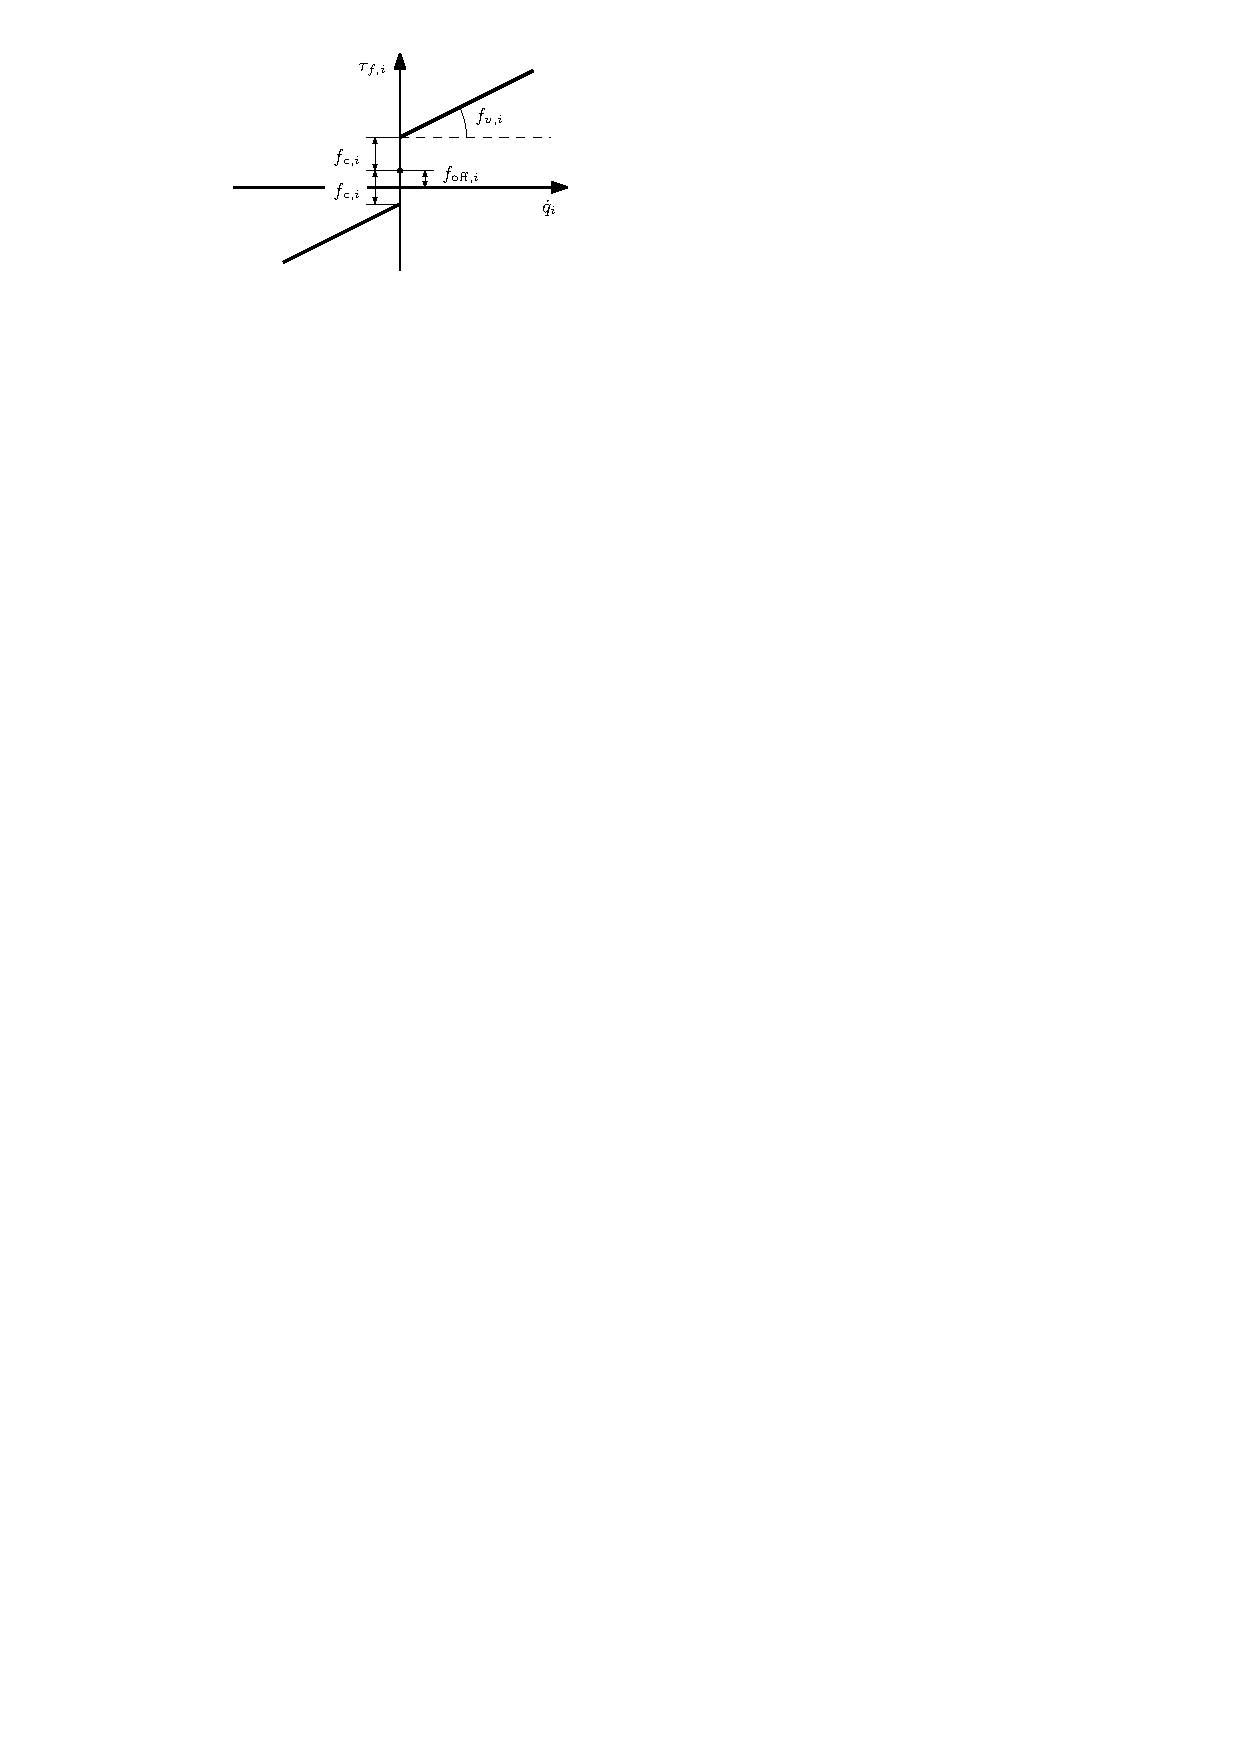
\includegraphics[width=0.7\textwidth]{friction_torque.pdf}
	\caption{График, поясняющий выбранную модель трения.}
	\label{img_friction_torque}
\end{figure}

Подставляя~\eqref{eq_friction_torque} в~\eqref{eq_eqs_with_tau_f}, получим
\begin{equation}
     \tau_e = I_a \ddot{q} + \xi \chi + f_v \dot{q} + f_c \sign(\dot{q}) + f_\text{off}\ldotp
\end{equation}
Если ввести в рассмотрение новые матрицы $\bar{\chi}=[\bar{\chi}_1, \: \bar\chi_2, \: \ldots, \: \bar\chi_5]^T$ и\linebreak
\begin{equation}
    \bar\xi =
    \begin{bmatrix}
        \bar\xi_{1,1} & \bar\xi_{1,2} & \cdots & \bar\xi_{1,5} \\
        O_{1 \times 10} & \bar\xi_{2,2} & \cdots & \bar\xi_{2,5} \\
        \vdots & \vdots & \ddots & \vdots \\
        O_{1 \times 10} & O_{1 \times 10} & O_{1 \times 10} & \bar\xi_{5,5}
    \end{bmatrix}\!\!,
\end{equation}
определяемые выражениями
\begin{equation}
    \bar{\chi}_i =
    \begin{bmatrix}
        \chi_i & I_{a,i} & f_{v,i} & f_{c,i} & f_{\text{off},i}
    \end{bmatrix}^T\!\!\!\!,
\end{equation}
\begin{equation}
    \bar{\xi}_{j,i} =
    \left\{
    \begin{aligned}
        \!\begin{bmatrix}\xi_{j,i} & 0 & 0 & 0 & 0\end{bmatrix}&, && i \ne j \\
        \!\begin{bmatrix}\xi_{j,i} & \ddot{q} & \dot{q} & \sign(\dot{q}) & 1\end{bmatrix}&, &&i = j
	\end{aligned}
	\right.
\end{equation}
то данное выражение может быть записано в следующем матричном виде:
\begin{equation}\label{eq_extended_dynamic_in_linear}
    \tau_e = \bar\xi \bar\chi \ldotp
\end{equation}

\subsubsection{Альтернативная матричная форма записи}
Выражение~\eqref{eq_dynamic_in_linear} может быть переписано в форме
\begin{equation}
    \tau = D(q) \ddot{q} + C(q,\dot{q}) \dot{q} + G(q),
\end{equation}
где $D(q)$~--- матрица инерции, $C(q,\dot{q})$~--- матрица центробежных и Кориолисовых сил, $G(q)$~--- вектор гравитации.
С~учетом этого факта и уравнения~\eqref{eq_eqs_with_tau_f} можно получить, что
\begin{equation}\label{eq_model_with_standard_matrix}
    \tau_e = M(q) \ddot{q} + C(q,\dot{q}) \dot{q} + G(q) + t_f(\dot{q}),
\end{equation}
где $M(q) = I_a + D(q)$.

Выражение для матрицы~$D(q)$ может быть найдено из формулы для кинетической энергии с учетом того, что справедливо
\begin{equation}\label{eq_K_in_form_with_D}
    K = \frac{1}{2} \, \dot{q}^T D(q) \dot{q},
\end{equation}
для матрицы $C(q,\dot{q})$~--- из выражения для $D(q)$ в соответствии с формулами:
\begin{gather}
    C_{ijk} = \cfrac{1}{2} \left( \cfrac{\partial D_{kj}}{\partial q_i} + \cfrac{\partial D_{ki}}{\partial q_j} - \cfrac{\partial D_{ij}}{\partial q_k}\right)\!\!,
    \\
    C_{kj} = \sum_{i = 1}^n C_{ijk} \dot{q}_i,
\end{gather}
где $D_{ij}$, $C_{ij}$~--- элементы матриц $D(q)$ и $C(q,\dot{q})$ соответственно, стоящие на пересечении $i$-ой строки и $j$-го столбца;
а для вектора $G(q)$~--- по формуле
\begin{equation}
    G(q) =
    \begin{bmatrix}
        \cfrac{\partial U}{\partial q_1} &
        \cfrac{\partial U}{\partial q_2} &
        \dots &
        \cfrac{\partial U}{\partial q_5}
    \end{bmatrix}^T\!\!\!\!\!\ldotp
\end{equation}

Выражение для кинетической энергии в форме~\eqref{eq_K_in_form_with_D} может быть получено из уравнения~\eqref{eq_eq_for_K_for_linear_model} с учетом формул~\eqref{eq_transform_of_g_v_omega}, \eqref{eq_work_of_lin_jacobians} и \eqref{eq_work_of_ang_jacobians}:
\begin{gather}
    K = \sum_{i=1}^5 \biggl( \frac{1}{2} m_i \cdot \left( {}^0R_i^T J_{vi} \dot{q} \right)^T \!\!\cdot \left({}^0R_i^T J_{vi} \dot{q}\right) + \frac{1}{2} \left( {}^0R_i^T J_{\omega i} \dot{q} \right)^T \!\!\cdot \mathcal{I}^{i}_i \cdot \left( {}^0R_i^T J_{\omega i} \dot{q} \right) + \notag\\
    %
    + (m_ir^i_{i,\,ci})^T \cdot \Bigl( \left( {}^0R_i^T J_{vi} \dot{q} \right) \times \left( {}^0R_i^T J_{\omega i} \dot{q} \right) \Bigr) \biggr) = \notag\\
    %
    = \sum_{i=1}^5 \biggl(\frac{1}{2} m_i \dot{q}^T J_{vi}^T J_{vi} \dot{q} \!+\! \frac{1}{2} \dot{q}^T J_{\omega i}^T \, {}^0\!R_i \, \mathcal{I}^{i}_i \, {}^0\!R_i^T J_{\omega i} \dot{q} \!+\! (m_i \underbrace{{}^0\!R_i r^i_{i,\,ci}}_{\displaystyle r^0_{i,\,ci}})^T \!\!\cdot \Bigl( \left( J_{vi} \dot{q} \right) \times \left( J_{\omega i} \dot{q} \right) \Bigr) \!\biggr) = \notag \\
    %
    = \frac{1}{2} \dot{q}^T \Biggl(\sum_{i=1}^5 \Bigl(m_i J_{vi}^T J_{vi} + J_{\omega i}^T \, {}^0\!R_i \, \mathcal{I}^{i}_i \, {}^0\!R_i^T J_{\omega i} + x\{ m_i r^0_{i,\,ci} \} \!\cdot\! J_{x} \,\, + \notag \\
    %
    + \,\, y\{ m_i r^0_{i,\,ci} \} \!\cdot\! J_{y} + z\{ m_i r^0_{i,\,ci} \} \!\cdot\! J_{z}\Bigr) \Biggr) \dot{q},
\end{gather}
при преобразованиях которого учтено то, что
\begin{equation*}
    \left( J_{vi} \dot{q} \right) \times \left( J_{\omega i} \dot{q} \right) =
    \begin{bmatrix}
        J_{vi}^{\{1\}} \dot{q}\\
        J_{vi}^{\{2\}} \dot{q}\\
        J_{vi}^{\{3\}} \dot{q}
    \end{bmatrix}
    \times
    \begin{bmatrix}
        J_{\omega i}^{\{1\}} \dot{q}\\
        J_{\omega i}^{\{2\}} \dot{q}\\
        J_{\omega i}^{\{3\}} \dot{q}
    \end{bmatrix}
    =
    \begin{bmatrix}
        -J_{vi}^{\{3\}} \dot{q} J_{\omega i}^{\{2\}} \dot{q} + J_{vi}^{\{2\}} \dot{q} J_{\omega i}^{\{3\}} \dot{q}\\
         J_{vi}^{\{3\}} \dot{q} J_{\omega i}^{\{1\}} \dot{q} - J_{vi}^{\{1\}} \dot{q} J_{\omega i}^{\{3\}} \dot{q}\\
        -J_{vi}^{\{2\}} \dot{q} J_{\omega i}^{\{1\}} \dot{q} + J_{vi}^{\{1\}} \dot{q} J_{\omega i}^{\{2\}} \dot{q}
    \end{bmatrix}
    =
\end{equation*}
\begin{equation}
    =
    \begin{bmatrix}
        -\dot{q}^T \bigl(J_{vi}^{\{3\}} \bigr)^T J_{\omega i}^{\{2\}} \dot{q} +
        \dot{q}^T \bigl( J_{vi}^{\{2\}} \bigr)^T J_{\omega i}^{\{3\}} \dot{q}
        \\
        \dot{q}^T \bigl( J_{vi}^{\{3\}} \bigr)^T J_{\omega i}^{\{1\}} \dot{q} -
        \dot{q}^T \bigl( J_{vi}^{\{1\}} \bigr)^T J_{\omega i}^{\{3\}} \dot{q}
        \\
        -\dot{q}^T \bigl( J_{vi}^{\{2\}} \bigr)^T J_{\omega i}^{\{1\}} \dot{q} +
        \dot{q}^T \bigl( J_{vi}^{\{1\}} \bigr)^T J_{\omega i}^{\{2\}} \dot{q}
    \end{bmatrix}
    =
    \begin{bmatrix}
        \dot{q}^T \! J_x \dot{q} \\
        \dot{q}^T \! J_y \dot{q} \\
        \dot{q}^T \! J_z \dot{q}
    \end{bmatrix}\!\!,
\end{equation}
где
\begin{align}
    &J_x =  - \bigl( J_{vi}^{\{3\}} \bigr)^T J_{\omega i}^{\{2\}} + \bigl( J_{vi}^{\{2\}} \bigr)^T J_{\omega i}^{\{3\}}, \\
    &J_y = \phantom{-}\bigl( J_{vi}^{\{3\}} \bigr)^T J_{\omega i}^{\{1\}} - \bigl( J_{vi}^{\{1\}} \bigr)^T J_{\omega i}^{\{3\}}, \\
    &J_z =  - \bigl( J_{vi}^{\{2\}} \bigr)^T J_{\omega i}^{\{1\}} + \bigl( J_{vi}^{\{1\}} \bigr)^T J_{\omega i}^{\{2\}} \ldotp
\end{align}
\newpage


\section{Синтез систем управления}\label{part_control_systems}
\subsection{Предварительные замечания}
Каждый из приводов манипулятора робота Kuka Youbot имеет собственную систему управления, структура которой иллюстрируется схемой с рисунка~\ref{img_structure_of_actuator_cs}.
Из нее видно, что каждый из приводов робота может управляться заданием значения для угла~$q_{di}$, или скорости~$\dot{q}_{di}$, или момента силы $\tau_{ed,i}$, который должен быть на нем обеспечен.
Это значение подается на вход соответствующего ПИД-регулятора, коэффициенты которого доступны настройке, и далее (уже в виде сигнала напряжения $u$)~--- на контролируемый двигатель.

\vspace{0.5cm}

\begin{figure}[h!]
	\centering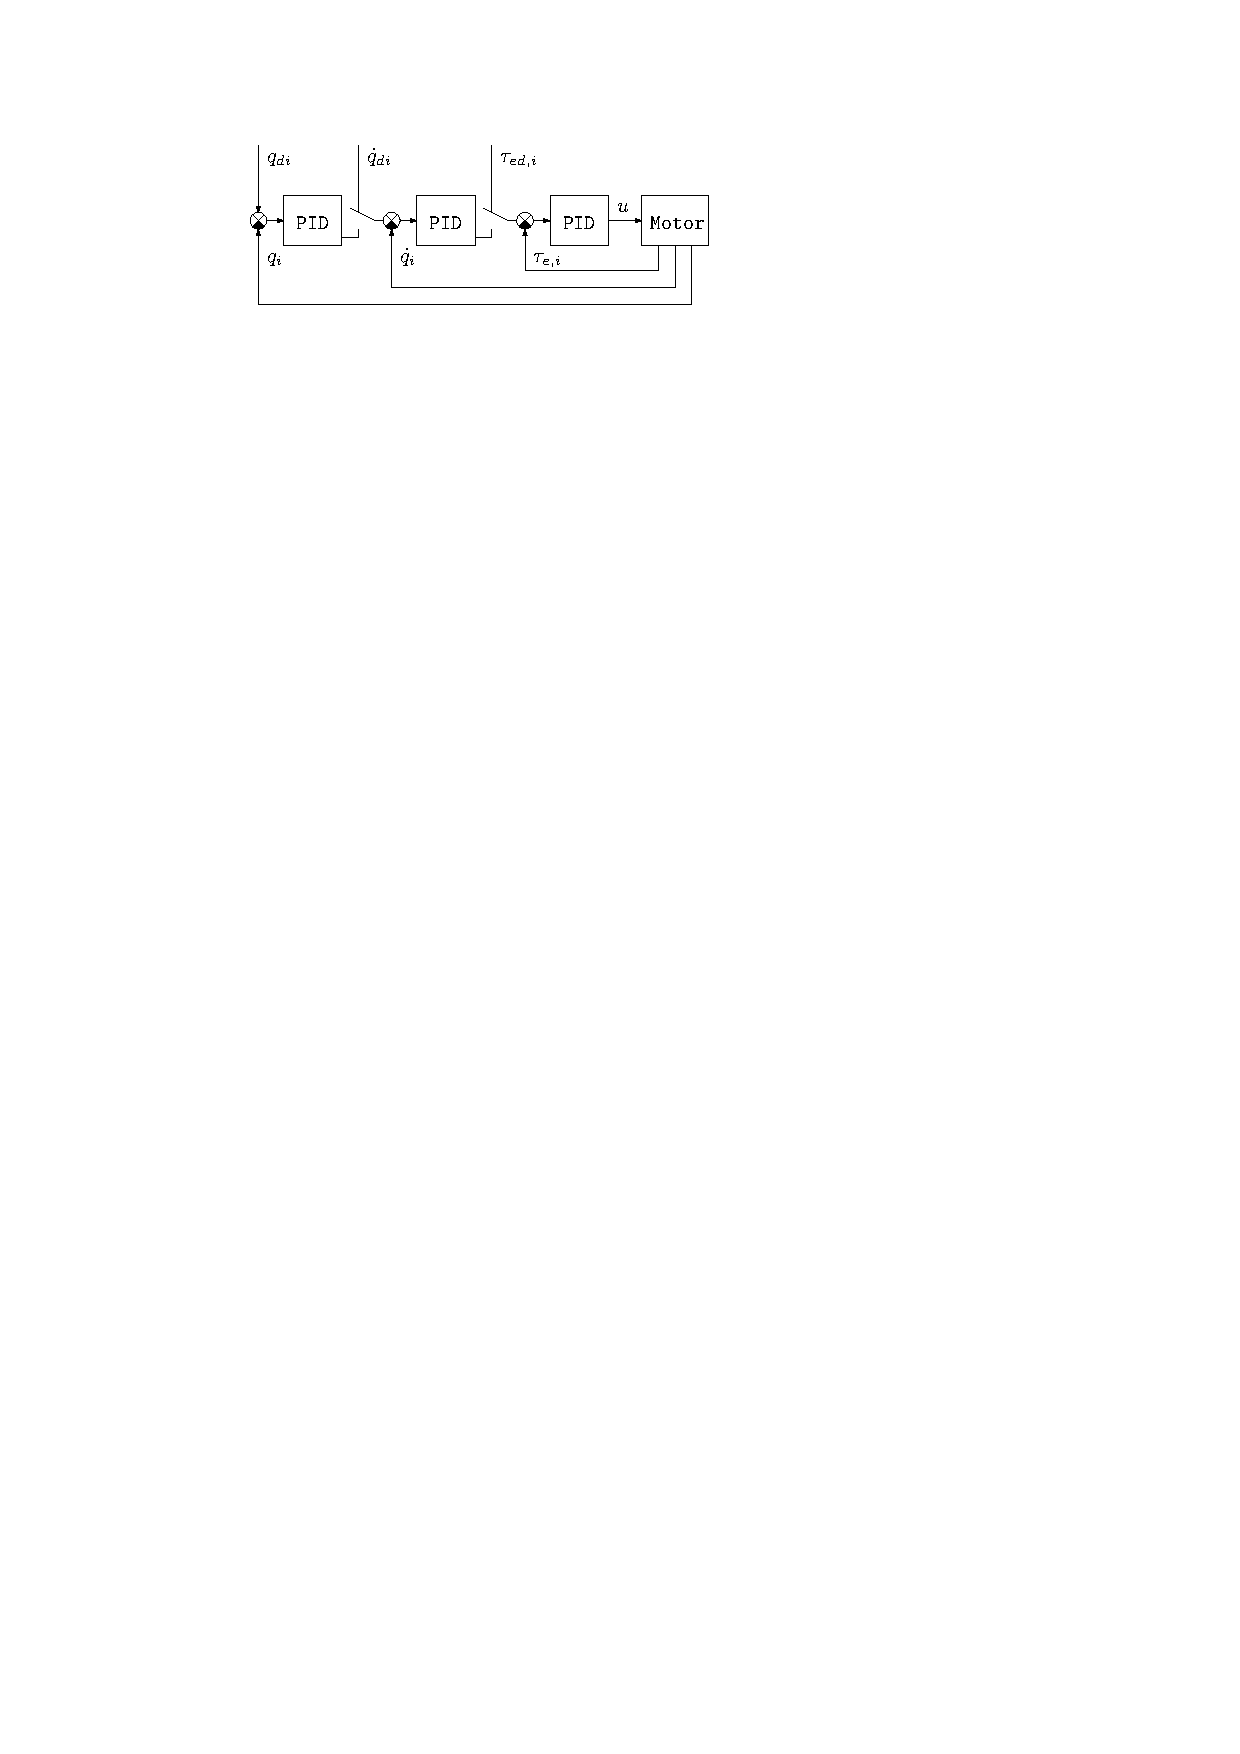
\includegraphics[width=0.8\textwidth]{structure_of_actuator_cs.pdf}
	\caption{Структура системы управления, контролирующей работу каждого из приводов робота.}
	\label{img_structure_of_actuator_cs}
\end{figure}

Далее в тексте документа будут рассмотрены системы управления, в которых в качестве управляющего сигнала рассматривается вектор $\tau_e(t)$.
При этом будет предполагаться, что задаваемые значения для моментов сил достигаются на двигателях мгновенно.
Такое предположение будем считать возможным по той причине, что процессы в контуре момента в рассмотренной выше системе управления характеризуются малыми временами переходных процессов.
В~качестве иллюстрации к сказанному можно привести рисунок~\ref{img_pid_transition_function}.
На нем показан график переходной функции системы управления моментом силы, развиваемым приводом ???-го звена.

\begin{figure}[h!]
	\centering\includegraphics[width=0.5\textwidth, draft]{pid_transition_function.pdf}
	\caption{График переходной функции системы управления приводом ???-го звена.}
	\label{img_pid_transition_function}
\end{figure}

Из величин, описывающих состояние робота в данный момент времени, в используемом ПО доступны вектора $q(t)$, $\dot{q}(t)$ и $\tau_e(t)$.

\subsection{Система управления для принятия определенной конфигурации}
Для системы управления процессом принятия роботом желаемой конфигурации, описываемой вектором $q_d = \left[ q_{d1} \; q_{d2} \; q_{d3} \; q_{d4} \; q_{d5} \right]^T = const$, выберем следующий закон управления:
\begin{equation}\label{eq_set_point_control_law}
    \tau_e = K_p (q_d - q) - K_d \dot{q} + G(q) + t_f(\dot{q}),
\end{equation}
где $K_p = \diag\{k_{pi}\} = const$ и $K_d = \diag\{k_{di}\} = const$, при этом $k_{pi}>0$ и $k_{di}>0$ для $\forall i=\overline{1,5}$.
С~учетом его и уравнения~\eqref{eq_model_with_standard_matrix} модель замкнутой системы примет вид:
\begin{equation}
    M(q) \ddot{q} + C(q,\dot{q}) \dot{q} = K_p (q_d - q) - K_d \dot{q}\ldotp
\end{equation}
Это выражение с использованием обозначений
\begin{equation}
    e = q - q_d,
    \qquad \qquad
    x =
    \begin{bmatrix}
        e \\ \dot{q}
    \end{bmatrix}\!\!,
\end{equation}
можно переписать следующим образом
\begin{equation}\label{eq_controlled_object_model}
    \dot{x} = f(x),
\end{equation}
где
\begin{equation}
    f(x) =
    \begin{bmatrix}
        \dot{q} \\
        -M^{-1}(e) \Bigl( K_p e + K_d \dot{q} + C(e,\dot{q}) \dot{q} \Bigr)
    \end{bmatrix}\!\!\ldotp
\end{equation}

Заметим, что равновесным состоянием системы~\eqref{eq_controlled_object_model} является точка \linebreak $x_0 = [0\;0\;\ldots\;0]^T$, так как $f(x_0) = [0\;0\;\ldots\;0]^T$.

Рассмотрим следующую функцию Ляпунова:
\begin{equation}
    V(x) = \frac{1}{2} \, \dot{q}^T \! M(e) \dot{q} + \frac{1}{2} \, e^T \! K_p e \ldotp
\end{equation}
Ее производная по времени\footnote{В~представленных ниже выкладках учтен тот факт, что матрица \linebreak $\bigl( 0.5 M(q) \bigr)^\centerdot \!\! - C(q,\dot{q})$ является кососимметричной.}
\begin{gather}
    \frac{d}{dt} V(x) = \dot{q}^T \! M(e) \ddot{q} + \dot{q}^T \frac{d}{dt} \Bigl( \frac{1}{2} M(e) \Bigr) \dot{q} + \dot{e}^T K_p e = \notag \\
    %
    = \dot{q}^T \Bigl( \tau_e - C(q,\dot{q}) \dot{q} - G(q) - t_f(\dot{q}) \Bigr) + \dot{q}^T \frac{d}{dt} \Bigl( \frac{1}{2} M(q) \Bigr) \dot{q} + \dot{q}^T K_p e  = \notag\\
    %
    = \dot{q}^T \Bigl( \tau_e - G(q) - t_f(\dot{q}) + K_p e\Bigr) + \dot{q}^T \biggl( \frac{d}{dt} \Bigl( \frac{1}{2} M(q) \Bigr) - C(q,\dot{q}) \biggr) \dot{q} = \notag \\
    %
    = \dot{q}^T \Bigl(K_p (q_d - q) - K_d \dot{q} + G(q) + t_f(\dot{q}) - G(q) - t_f(\dot{q}) + K_p (q - q_d) \Bigr) = \notag \\
    %
    = -\dot{q}^T K_d \dot{q} < 0
\end{gather}
при $x \ne x_0$ и равна нулю при $x = x_0$.
Следовательно, по 2-ой теореме Ляпунова состояние системы $x = x_0$, при котором, к слову сказать, $q = q_d$ и $\dot{q} = [0\;0\;\ldots\;0]^T$, является асимптотически устойчивым.

\subsection{Система управления процессом следования по траектории}
Для системы управления процессом следования роботом по траектории, описываемой вектор-функцией $q_d(t) = \left[ q_{d1}(t) \; q_{d2}(t) \; q_{d3}(t) \; q_{d4}(t) \; q_{d5}(t) \right]^T$\!\!\!,\; возьмем следующий закон управления:
\begin{equation}\label{eq_trajectory_tracking_control_law}
    \tau_e = M(q) \bigl( \ddot{q}_d + K_d (\dot{q}_d - \dot{q})+  K_p (q_d - q) \bigr) + C(q,\dot{q}) \dot{q} + G(q) + t_f(\dot{q}),
\end{equation}
где $K_d = const$ и $K_p = const$.

С~учетом его и уравнения~\eqref{eq_model_with_standard_matrix} модель замкнутой системы опишется следующим выражением:
\begin{equation}
    M(q) \bigl( \ddot{q}_d - \ddot{q} + K_d (\dot{q}_d - \dot{q})+  K_p (q_d - q) \bigr) = 0,
\end{equation}
которое после деления на $M(q)$ и применения обозначения
\begin{equation}
    \varepsilon = q_d - q
\end{equation}
может быть переписано в виде:
\begin{equation}\label{eq_trajectory_tracking_closed_loop}
    \ddot{\varepsilon} + K_d \dot{\varepsilon} +  K_p \varepsilon = 0 \ldotp
\end{equation}

Согласно последнему уравнению, использование закона управления~\eqref{eq_trajectory_tracking_control_law} дает возможность полностью определять поведение робота значениями матриц $K_p$ и $K_d$.

В~данной работе матрицы $K_p$ и $K_d$ были выбраны диагональными:
\begin{equation}
    K_p = \diag\{k_{pi}\},
    \qquad
    K_d = \diag\{k_{di}\},
\end{equation}
потому что это позволяет <<разбить>> уравнение~\eqref{eq_trajectory_tracking_closed_loop} на 5~независимых дифференциальных уравнений, а их компоненты~--- положительными:
\begin{equation}
    \qquad
    k_{pi} > 0,\ k_{di} > 0,\ \forall i=\overline{1,5},
\end{equation}
так как при этом система получается устойчивой (все 5~уравнений получаются имеющими корни только с отрицательной вещественной частью).

\newpage

\section*{Заключение}
\addcontentsline{toc}{section}{Заключение}
Текст заключения
\newpage
\renewcommand\refname{Список использованных источников}
\providecommand*{\url}[1]{#1} %нужно для описания некоторых источников
\bibliography{used_books}
\ESKDappendix{рекомендуемое}{Матрицы однородного преобразования}\label{app_ht_matrices}
Матрицей однородного преобразования ${}^{i}A_j$ называется матрица размера $4 \times 4$, служащая для описания смещения и поворота СК $Ox_{j}y_{j}z_{j}$ относительно СК $Ox_{i}y_{i}z_{i}$ и имеющая следующую структуру:
\begin{equation}
    {}^{i}A_j =
    \begin{bmatrix}
        {}^{i}R_j & r^{i}_{i,\,j}\\
        O_{1 \times 3} & 1
    \end{bmatrix}\!\!,
\end{equation}
где $O_{1 \times 3} = [0\;0\;0]$.

Принципы ее использования поясняет следующий пример.

Рассмотрим рисунок~\ref{img:three_frames}.
Чтобы найти координаты точки~$C$ относительно $Ox_0y_0z_0$ при известных векторах $r^2_C$, $r^{0}_{0,\,1}$ и $r^{1}_{1,\,2}$ и поворотах всех СК друг относительно друга,  могут быть использованы следующие выражения:
\begin{equation}
	\left\{
	\begin{aligned}
		\!&r^0_C = {}^{0}R_1 r^1_C + r^{0}_{0,\,1}\\
		\!&r^1_C = {}^{1}R_2 r^2_C + r^{1}_{1,\,2}
	\end{aligned}
	\right.
	\quad \Rightarrow \quad
	r^0_C = {}^{0}R_1{}^{1}R_2 r^2_C + {}^{0}R_1 r^{1}_{1,\,2} + r^{0}_{0,\,1}
\end{equation}
где $r^0_C$, $r^1_C$, $r^2_C$~--- радиус-векторы точки~$C$ в $Ox_0y_0z_0$, $Ox_1y_1z_1$ и $Ox_2y_2z_2$ соответственно.
В~это же время можно воспользоваться и матрицами ${}^{0}A_1$ и ${}^{1}A_2$:
\begin{multline}
	\left\{
	\begin{aligned}
		\!&\begin{bmatrix}r^0_C \\ 1\end{bmatrix} = \underbrace{\begin{bmatrix} {}^{0}R_1 & r^{0}_{0,\,1}\\ O_{1 \times 3} & 1 \end{bmatrix}}_{{}^{0}A_1}\begin{bmatrix}r^1_C \\ 1\end{bmatrix} = \begin{bmatrix}{}^{0}R_1 r^1_C + r^{0}_{0,\,1} \\ 1\end{bmatrix}\\
		\!&\begin{bmatrix}r^1_C \\ 1\end{bmatrix} = \underbrace{\begin{bmatrix} {}^{1}R_2 & r^{1}_{1,\,2}\\ O_{1 \times 3} & 1 \end{bmatrix}}_{{}^{1}A_2}\begin{bmatrix}r^2_C \\ 1\end{bmatrix} = \begin{bmatrix}{}^{1}R_2 r^2_C + r^{1}_{1,\,2} \\ 1\end{bmatrix}
	\end{aligned}
	\right.
	\quad \Rightarrow
	\\
	\Rightarrow \quad
	\begin{bmatrix}r^0_C \\ 1\end{bmatrix} = \underbrace{\underbrace{\begin{bmatrix} {}^{0}R_1 & r^{0}_{0,\,1}\\ O_{1 \times 3} & 1 \end{bmatrix}}_{{}^{0}A_1}\underbrace{\begin{bmatrix} {}^{1}R_2 & r^{1}_{1,\,2}\\ O_{1 \times 3} & 1 \end{bmatrix}}_{{}^{1}A_2}}_{{}^{0}A_2} \begin{bmatrix}r^2_C \\ 1\end{bmatrix} = \underbrace{\begin{bmatrix} {}^{0}R_1 & r^{0}_{0,\,1}\\ O_{1 \times 3} & 1 \end{bmatrix}}_{{}^{0}A_1} \begin{bmatrix}{}^{1}R_2 r^2_C + r^{1}_{1,\,2} \\ 1\end{bmatrix} =\\
	= \begin{bmatrix}{}^{0}R_1{}^{1}R_2 r^2_C + {}^{0}R_1 r^{1}_{1,\,2} + r^{0}_{0,\,1} \\ 1\end{bmatrix}
\end{multline}

Дополнительная информация о матрицах однородного преобразования доступна, например, в~\cite{}.

\begin{figure}[h!]
	\centering
	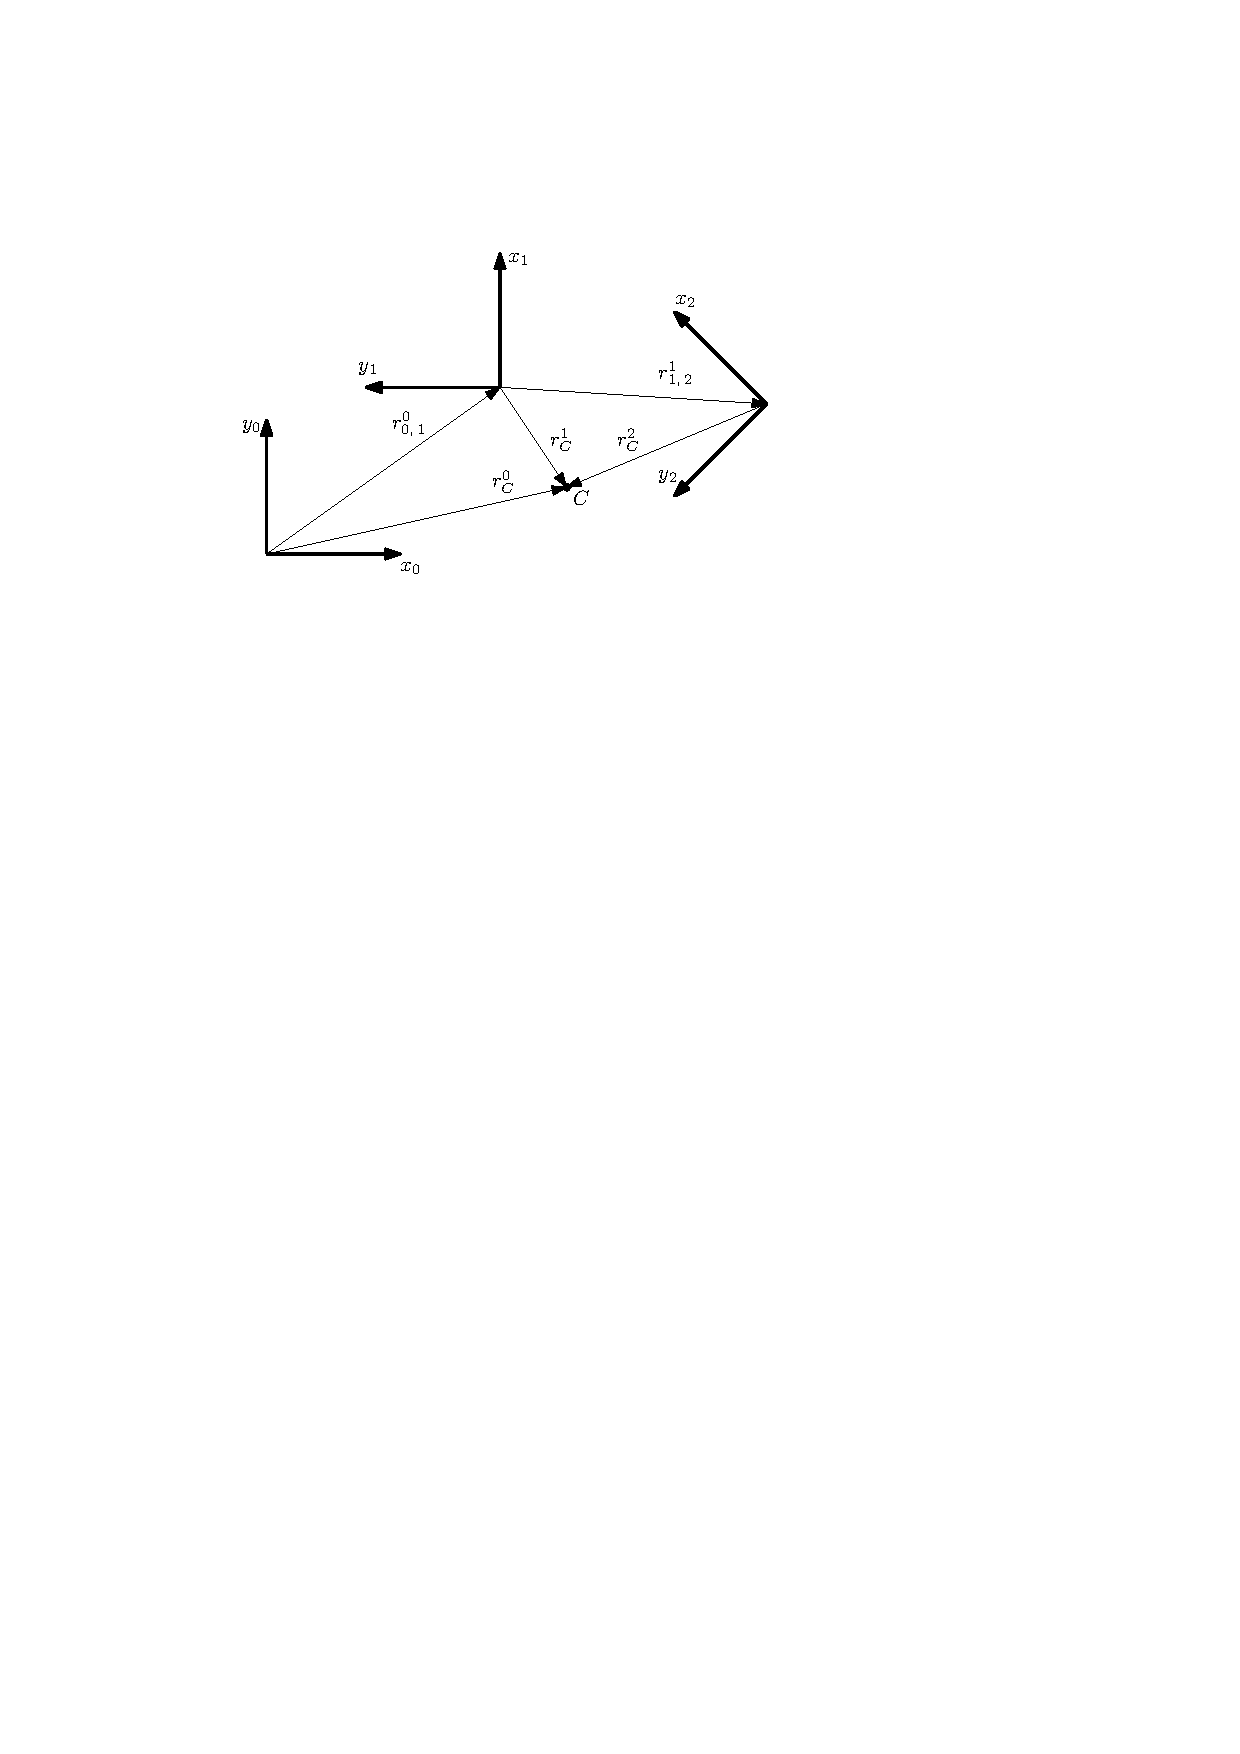
\includegraphics[width=0.7\textwidth]{three_frames.pdf}
	\caption{Системы координат из пояснительного примера.}
	\label{img:three_frames}
\end{figure}
\ESKDappendix{рекомендуемое}{Терминология относительных измерений}\label{app_relative_relativity}
Относительно координат некоторых векторов, являющихся в большинстве своем некоторыми кинематическими величинами, в тексте документа можно встретить указания на то, что они получены (или отсчитаны) <<\dots относитель\-но такой-то системы координат\dots>> и при этом <<\dots выражены относительно такой-то системы координат\dots>>.
Это приложение разъясняет смысл данных фраз нижеследующим простым примером.

Рассмотрим рисунок~\ref{img:tree_cart_and_bird}.
На нем изображены стоящий неподвижно куст, тележка, катящаяся со скоростью $v=1\text{ м/с}$, облако, движущееся со скоростью $u=3\text{ м/с}$, и жестко связанные с ними правосторонние системы координат $Ox_0y_0z_0$, $Ox_1y_1z_1$ и $Ox_2y_2z_2$.
Опишем скорость движения облака вектором~$V$.
В~зависимости от своего физического смысла он будет иметь разные координаты.
Наглядно это демонстрирует таблица~\ref{table_values_of_v}.

\begin{figure}[h!]
	\centering
	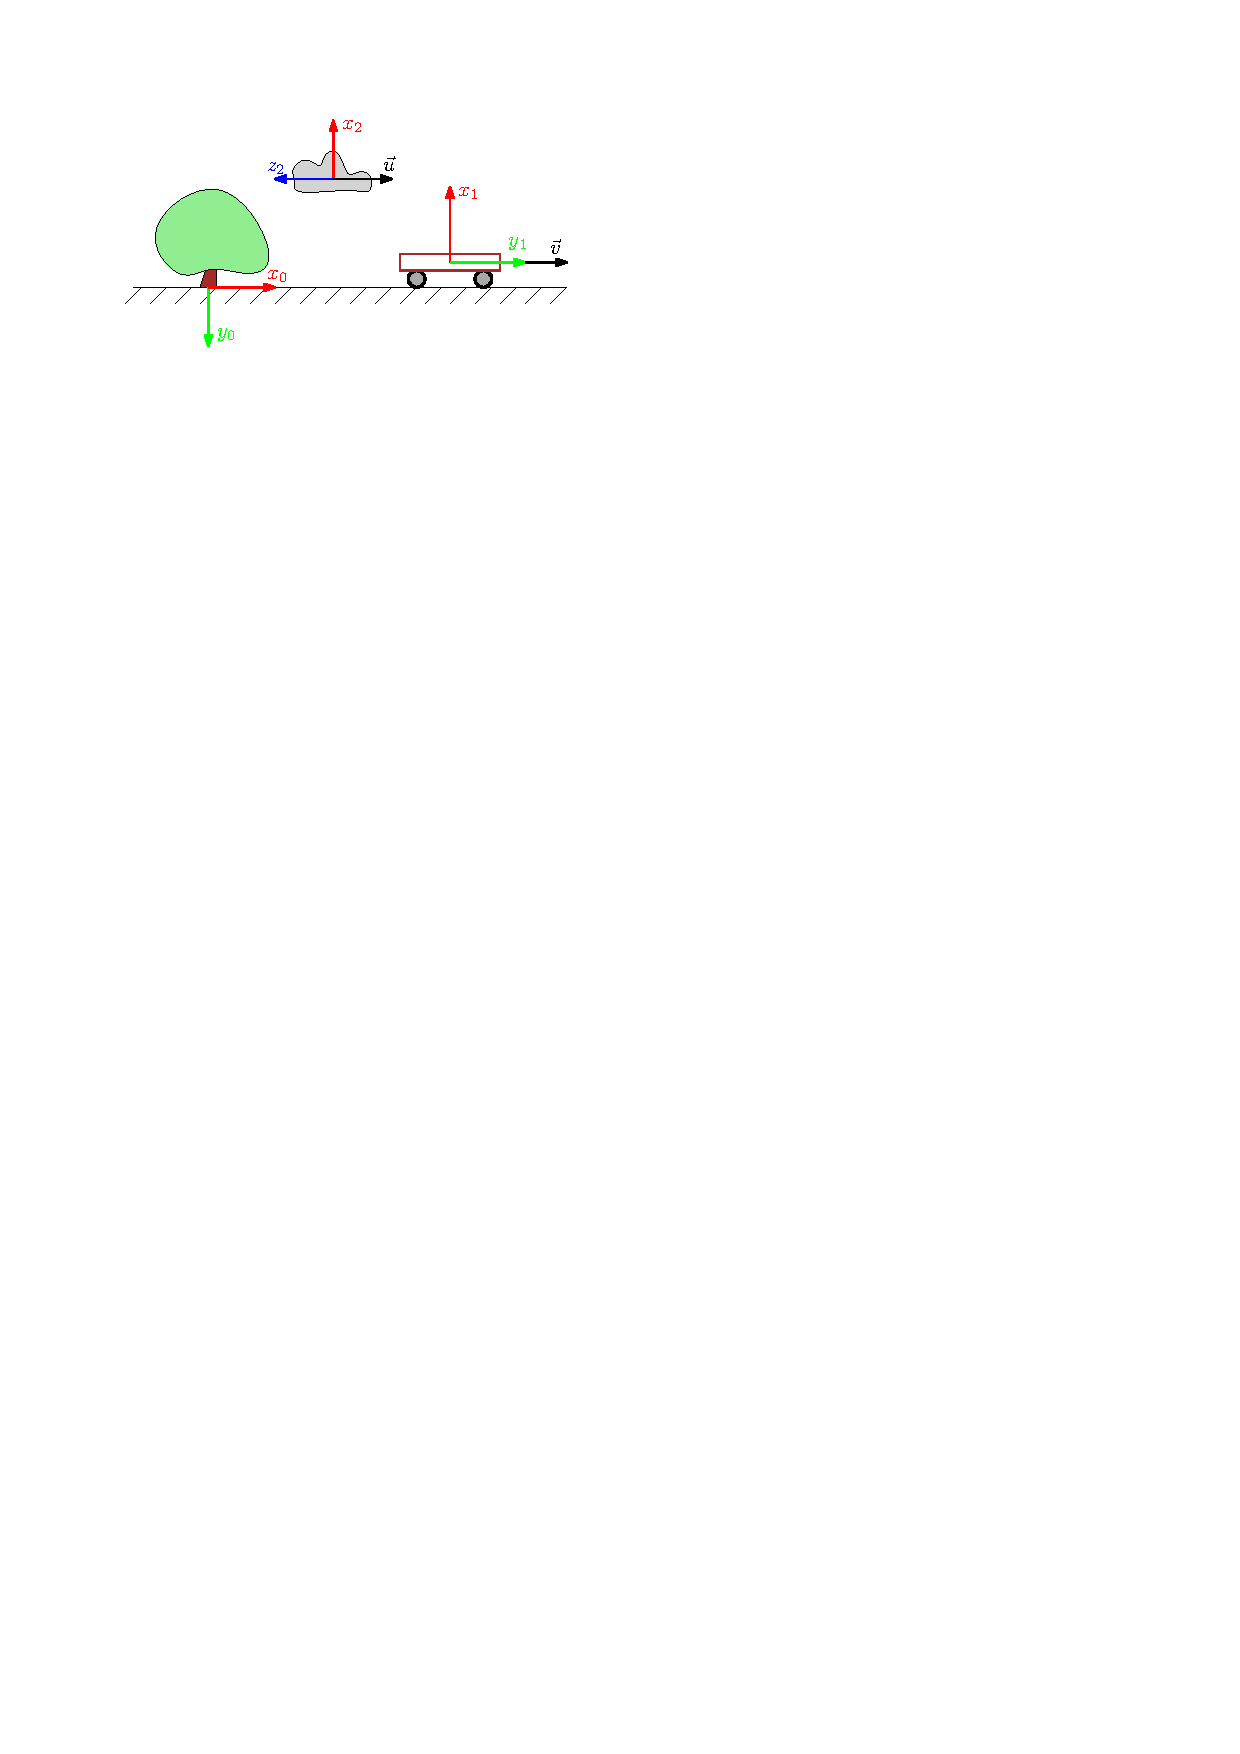
\includegraphics[width=0.9\textwidth]{tree_cart_and_bird.pdf}
	\caption{Воображаемая ситуация из пояснительного примера.}
	\label{img:tree_cart_and_bird}
\end{figure}

\begin{table}[h!]
	\caption{Координаты вектора $V$ в зависимости от его физического смысла.}
	\begin{center}
		\begin{tabular}{|m{13cm}|m{3cm}|}
			\hline
			\multicolumn{1}{|c|}{Смысл вектора $V$} & \makebox[3cm]{Значение $V^T$}\\
			\hline
			Скорость $Ox_2y_2z_2$ относительно $Ox_0y_0z_0$, выраженная относительно $Ox_0y_0z_0$ & $$\begin{bmatrix}3 & 0 & 0\end{bmatrix}$$\\
			\hline
			Скорость $Ox_2y_2z_2$ относительно $Ox_0y_0z_0$, выраженная относительно $Ox_1y_1z_1$ & $$\begin{bmatrix}0 & 3 & 0\end{bmatrix}$$\\
			\hline
			Скорость $Ox_2y_2z_2$ относительно $Ox_0y_0z_0$, выраженная относительно $Ox_2y_2z_2$ & $$\begin{bmatrix}0 & 0 & -3\end{bmatrix}$$\\
			\hline
			Скорость $Ox_2y_2z_2$ относительно $Ox_1y_1z_1$, выраженная относительно $Ox_0y_0z_0$ & $$\begin{bmatrix}2 & 0 & 0\end{bmatrix}$$\\
			\hline
			Скорость $Ox_2y_2z_2$ относительно $Ox_1y_1z_1$, выраженная относительно $Ox_1y_1z_1$ & $$\begin{bmatrix}0 & 2 & 0\end{bmatrix}$$\\
			\hline
			Скорость $Ox_2y_2z_2$ относительно $Ox_1y_1z_1$, выраженная относительно $Ox_2y_2z_2$ & $$\begin{bmatrix}0 & 0 & -2\end{bmatrix}$$\\
			\hline
		\end{tabular}
	\end{center}
	\label{table_values_of_v}
\end{table}


\end{document}
